\documentclass[twoside]{book}

% Packages required by doxygen
\usepackage{fixltx2e}
\usepackage{calc}
\usepackage{doxygen}
\usepackage[export]{adjustbox} % also loads graphicx
\usepackage{graphicx}
\usepackage[utf8]{inputenc}
\usepackage{makeidx}
\usepackage{multicol}
\usepackage{multirow}
\PassOptionsToPackage{warn}{textcomp}
\usepackage{textcomp}
\usepackage[nointegrals]{wasysym}
\usepackage[table]{xcolor}

% NLS support packages
\usepackage[french]{babel}

% Font selection
\usepackage[T1]{fontenc}
\usepackage[scaled=.90]{helvet}
\usepackage{courier}
\usepackage{amssymb}
\usepackage{sectsty}
\renewcommand{\familydefault}{\sfdefault}
\allsectionsfont{%
  \fontseries{bc}\selectfont%
  \color{darkgray}%
}
\renewcommand{\DoxyLabelFont}{%
  \fontseries{bc}\selectfont%
  \color{darkgray}%
}
\newcommand{\+}{\discretionary{\mbox{\scriptsize$\hookleftarrow$}}{}{}}

% Page & text layout
\usepackage{geometry}
\geometry{%
  a4paper,%
  top=2.5cm,%
  bottom=2.5cm,%
  left=2.5cm,%
  right=2.5cm%
}
\tolerance=750
\hfuzz=15pt
\hbadness=750
\setlength{\emergencystretch}{15pt}
\setlength{\parindent}{0cm}
\setlength{\parskip}{3ex plus 2ex minus 2ex}
\makeatletter
\renewcommand{\paragraph}{%
  \@startsection{paragraph}{4}{0ex}{-1.0ex}{1.0ex}{%
    \normalfont\normalsize\bfseries\SS@parafont%
  }%
}
\renewcommand{\subparagraph}{%
  \@startsection{subparagraph}{5}{0ex}{-1.0ex}{1.0ex}{%
    \normalfont\normalsize\bfseries\SS@subparafont%
  }%
}
\makeatother

% Headers & footers
\usepackage{fancyhdr}
\pagestyle{fancyplain}
\fancyhead[LE]{\fancyplain{}{\bfseries\thepage}}
\fancyhead[CE]{\fancyplain{}{}}
\fancyhead[RE]{\fancyplain{}{\bfseries\leftmark}}
\fancyhead[LO]{\fancyplain{}{\bfseries\rightmark}}
\fancyhead[CO]{\fancyplain{}{}}
\fancyhead[RO]{\fancyplain{}{\bfseries\thepage}}
\fancyfoot[LE]{\fancyplain{}{}}
\fancyfoot[CE]{\fancyplain{}{}}
\fancyfoot[RE]{\fancyplain{}{\bfseries\scriptsize Généré par Doxygen }}
\fancyfoot[LO]{\fancyplain{}{\bfseries\scriptsize Généré par Doxygen }}
\fancyfoot[CO]{\fancyplain{}{}}
\fancyfoot[RO]{\fancyplain{}{}}
\renewcommand{\footrulewidth}{0.4pt}
\renewcommand{\chaptermark}[1]{%
  \markboth{#1}{}%
}
\renewcommand{\sectionmark}[1]{%
  \markright{\thesection\ #1}%
}

% Indices & bibliography
\usepackage{natbib}
\usepackage[titles]{tocloft}
\setcounter{tocdepth}{3}
\setcounter{secnumdepth}{5}
\makeindex

% Hyperlinks (required, but should be loaded last)
\usepackage{ifpdf}
\ifpdf
  \usepackage[pdftex,pagebackref=true]{hyperref}
\else
  \usepackage[ps2pdf,pagebackref=true]{hyperref}
\fi
\hypersetup{%
  colorlinks=true,%
  linkcolor=blue,%
  citecolor=blue,%
  unicode%
}

% Custom commands
\newcommand{\clearemptydoublepage}{%
  \newpage{\pagestyle{empty}\cleardoublepage}%
}

\usepackage{caption}
\captionsetup{labelsep=space,justification=centering,font={bf},singlelinecheck=off,skip=4pt,position=top}

%===== C O N T E N T S =====

\begin{document}

% Titlepage & ToC
\hypersetup{pageanchor=false,
             bookmarksnumbered=true,
             pdfencoding=unicode
            }
\pagenumbering{alph}
\begin{titlepage}
\vspace*{7cm}
\begin{center}%
{\Large Atlantik \\[1ex]\large 1.\+0 beta 1 }\\
\vspace*{1cm}
{\large Généré par Doxygen 1.8.13}\\
\end{center}
\end{titlepage}
\clearemptydoublepage
\pagenumbering{roman}
\tableofcontents
\clearemptydoublepage
\pagenumbering{arabic}
\hypersetup{pageanchor=true}

%--- Begin generated contents ---
\chapter{Index des espaces de nommage}
\section{Liste des espaces de nommage}
Liste de tous les espaces de nommage avec une brève description\+:\begin{DoxyCompactList}
\item\contentsline{section}{\hyperlink{namespace_ui}{Ui} }{\pageref{namespace_ui}}{}
\end{DoxyCompactList}

\chapter{Index hiérarchique}
\section{Hiérarchie des classes}
Cette liste d\textquotesingle{}héritage est classée approximativement par ordre alphabétique \+:\begin{DoxyCompactList}
\item \contentsline{section}{Bateau}{\pageref{class_bateau}}{}
\begin{DoxyCompactList}
\item \contentsline{section}{Bateau\+Voyageur}{\pageref{class_bateau_voyageur}}{}
\end{DoxyCompactList}
\item \contentsline{section}{Equipement}{\pageref{class_equipement}}{}
\item \contentsline{section}{Passerelle}{\pageref{class_passerelle}}{}
\item Q\+Main\+Window\begin{DoxyCompactList}
\item \contentsline{section}{Main\+Window}{\pageref{class_main_window}}{}
\end{DoxyCompactList}
\item Q\+Sql\+Query\begin{DoxyCompactList}
\item \contentsline{section}{Jeu\+Enregistrement}{\pageref{class_jeu_enregistrement}}{}
\end{DoxyCompactList}
\item Q\+Text\+Browser\begin{DoxyCompactList}
\item \contentsline{section}{P\+DF}{\pageref{class_p_d_f}}{}
\end{DoxyCompactList}
\end{DoxyCompactList}

\chapter{Index des classes}
\section{Liste des classes}
Liste des classes, structures, unions et interfaces avec une brève description \+:\begin{DoxyCompactList}
\item\contentsline{section}{\hyperlink{class_bateau}{Bateau} \\*La classe \hyperlink{class_bateau}{Bateau} C\textquotesingle{}est la classe mère de la classe \hyperlink{class_bateau_voyageur}{Bateau\+Voyageur} Chaque bateau dispose de 4 propriétés }{\pageref{class_bateau}}{}
\item\contentsline{section}{\hyperlink{class_bateau_voyageur}{Bateau\+Voyageur} \\*La classe \hyperlink{class_bateau_voyageur}{Bateau\+Voyageur} C\textquotesingle{}est une dépendance de la classe \hyperlink{class_passerelle}{Passerelle} Chaque bateau voyageur dispose de 3 propriétés }{\pageref{class_bateau_voyageur}}{}
\item\contentsline{section}{\hyperlink{class_equipement}{Equipement} \\*La classe \hyperlink{class_equipement}{Equipement} C\textquotesingle{}est une dépendance de la classe \hyperlink{class_passerelle}{Passerelle} Chaque équipement possède 2 propriétés }{\pageref{class_equipement}}{}
\item\contentsline{section}{\hyperlink{class_jeu_enregistrement}{Jeu\+Enregistrement} \\*La classe \hyperlink{class_jeu_enregistrement}{Jeu\+Enregistrement} Elle hérite de la classe Q\+Sql\+Query Elle permet de manipuler un jeu de données }{\pageref{class_jeu_enregistrement}}{}
\item\contentsline{section}{\hyperlink{class_main_window}{Main\+Window} \\*La classe \hyperlink{class_main_window}{Main\+Window} Elle hérite de la classe Q\+Main\+Window Elle permet de créer la fenêtre de l\textquotesingle{}application }{\pageref{class_main_window}}{}
\item\contentsline{section}{\hyperlink{class_passerelle}{Passerelle} \\*La classe \hyperlink{class_passerelle}{Passerelle} Elle est dépendante des classes \hyperlink{class_bateau_voyageur}{Bateau\+Voyageur} et \hyperlink{class_equipement}{Equipement} }{\pageref{class_passerelle}}{}
\item\contentsline{section}{\hyperlink{class_p_d_f}{P\+DF} \\*La classe \hyperlink{class_p_d_f}{P\+DF} Elle hérite de la classe Q\+Text\+Browser Elle permet de générer un document \hyperlink{class_p_d_f}{P\+DF} Chaque pdf d\textquotesingle{}une propriété }{\pageref{class_p_d_f}}{}
\end{DoxyCompactList}

\chapter{Index des fichiers}
\section{Liste des fichiers}
Liste de tous les fichiers avec une brève description \+:\begin{DoxyCompactList}
\item\contentsline{section}{\hyperlink{bateau_8cpp}{bateau.\+cpp} }{\pageref{bateau_8cpp}}{}
\item\contentsline{section}{\hyperlink{bateau_8h}{bateau.\+h} }{\pageref{bateau_8h}}{}
\item\contentsline{section}{\hyperlink{bateauvoyageur_8cpp}{bateauvoyageur.\+cpp} }{\pageref{bateauvoyageur_8cpp}}{}
\item\contentsline{section}{\hyperlink{bateauvoyageur_8h}{bateauvoyageur.\+h} }{\pageref{bateauvoyageur_8h}}{}
\item\contentsline{section}{\hyperlink{equipement_8cpp}{equipement.\+cpp} }{\pageref{equipement_8cpp}}{}
\item\contentsline{section}{\hyperlink{equipement_8h}{equipement.\+h} }{\pageref{equipement_8h}}{}
\item\contentsline{section}{\hyperlink{jeuenregistrement_8cpp}{jeuenregistrement.\+cpp} }{\pageref{jeuenregistrement_8cpp}}{}
\item\contentsline{section}{\hyperlink{jeuenregistrement_8h}{jeuenregistrement.\+h} }{\pageref{jeuenregistrement_8h}}{}
\item\contentsline{section}{\hyperlink{main_8cpp}{main.\+cpp} }{\pageref{main_8cpp}}{}
\item\contentsline{section}{\hyperlink{mainwindow_8cpp}{mainwindow.\+cpp} }{\pageref{mainwindow_8cpp}}{}
\item\contentsline{section}{\hyperlink{mainwindow_8h}{mainwindow.\+h} }{\pageref{mainwindow_8h}}{}
\item\contentsline{section}{\hyperlink{passerelle_8cpp}{passerelle.\+cpp} }{\pageref{passerelle_8cpp}}{}
\item\contentsline{section}{\hyperlink{passerelle_8h}{passerelle.\+h} }{\pageref{passerelle_8h}}{}
\item\contentsline{section}{\hyperlink{pdf_8cpp}{pdf.\+cpp} }{\pageref{pdf_8cpp}}{}
\item\contentsline{section}{\hyperlink{pdf_8h}{pdf.\+h} }{\pageref{pdf_8h}}{}
\end{DoxyCompactList}

\chapter{Documentation des espaces de nommage}
\hypertarget{namespace_ui}{}\section{Référence de l\textquotesingle{}espace de nommage Ui}
\label{namespace_ui}\index{Ui@{Ui}}


\subsection{Description détaillée}
\begin{DoxyAuthor}{Auteur}
Louis Vraie 
\end{DoxyAuthor}
\begin{DoxyDate}{Date}
08/11/2021 
\end{DoxyDate}
\begin{DoxyVersion}{Version}
1.\+0 beta 1 
\end{DoxyVersion}
\begin{DoxyCopyright}{Copyright}
G\+NU Public License 
\end{DoxyCopyright}

\chapter{Documentation des classes}
\hypertarget{class_bateau}{}\section{Référence de la classe Bateau}
\label{class_bateau}\index{Bateau@{Bateau}}


La classe \hyperlink{class_bateau}{Bateau} C\textquotesingle{}est la classe mère de la classe \hyperlink{class_bateau_voyageur}{Bateau\+Voyageur} Chaque bateau dispose de 4 propriétés.  




{\ttfamily \#include $<$bateau.\+h$>$}



Graphe d\textquotesingle{}héritage de Bateau\+:\nopagebreak
\begin{figure}[H]
\begin{center}
\leavevmode
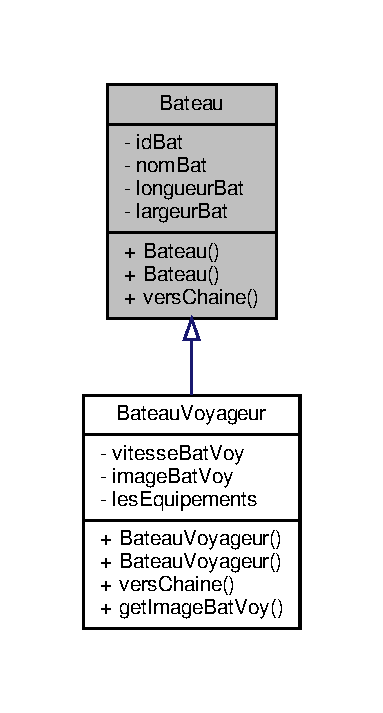
\includegraphics[width=184pt]{class_bateau__inherit__graph}
\end{center}
\end{figure}


Graphe de collaboration de Bateau\+:\nopagebreak
\begin{figure}[H]
\begin{center}
\leavevmode
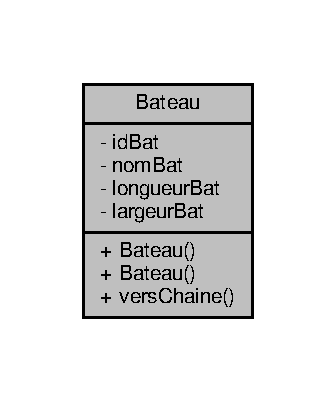
\includegraphics[width=161pt]{class_bateau__coll__graph}
\end{center}
\end{figure}
\subsection*{Fonctions membres publiques}
\begin{DoxyCompactItemize}
\item 
\hyperlink{class_bateau_a5ea29ce02b632a199385200248a05581}{Bateau} (Q\+String un\+Id, Q\+String un\+Nom, float une\+Longueur, float une\+Largeur)
\begin{DoxyCompactList}\small\item\em \hyperlink{class_bateau_a5ea29ce02b632a199385200248a05581}{Bateau\+::\+Bateau} Constructeur de la classe \hyperlink{class_bateau}{Bateau} qui permet de remplir les propriétés privées du bateau avec les valeurs passées en paramètre. \end{DoxyCompactList}\item 
\hyperlink{class_bateau_a9b2027f6f3a71d6b05209e22b928db00}{Bateau} ()
\begin{DoxyCompactList}\small\item\em \hyperlink{class_bateau_a5ea29ce02b632a199385200248a05581}{Bateau\+::\+Bateau} Constructeur vide de la classe \hyperlink{class_bateau}{Bateau} nécessaire car il y a des vecteurs de \hyperlink{class_bateau}{Bateau}. \end{DoxyCompactList}\item 
Q\+String \hyperlink{class_bateau_a392f6a45649a2a35186dfcd1ca58eddc}{vers\+Chaine} ()
\begin{DoxyCompactList}\small\item\em \hyperlink{class_bateau_a392f6a45649a2a35186dfcd1ca58eddc}{Bateau\+::vers\+Chaine} Cette méthode publique renvoie la chaîne de caractère utilisée pour décrire le bateau~\newline
Exemple \+:~\newline
Nom du bateau \+: Queen Mary~\newline
Longueur \+: 14.\+5 mètres~\newline
Largeur \+: 8.\+2 mètres. \end{DoxyCompactList}\end{DoxyCompactItemize}
\subsection*{Attributs privés}
\begin{DoxyCompactItemize}
\item 
Q\+String \hyperlink{class_bateau_acf710114558ee740be62211df06133e1}{id\+Bat}
\item 
Q\+String \hyperlink{class_bateau_a2d01e3edfc60cb9111a5f4f11b2813b3}{nom\+Bat}
\item 
float \hyperlink{class_bateau_a6c1f8f9f5bb656fae6ce59bcfa6fe8aa}{longueur\+Bat}
\item 
float \hyperlink{class_bateau_ace3ced3b9bb6506a913645230b85022c}{largeur\+Bat}
\end{DoxyCompactItemize}


\subsection{Description détaillée}
La classe \hyperlink{class_bateau}{Bateau} C\textquotesingle{}est la classe mère de la classe \hyperlink{class_bateau_voyageur}{Bateau\+Voyageur} Chaque bateau dispose de 4 propriétés. 

\begin{DoxyAuthor}{Auteur}
Louis Vraie 
\end{DoxyAuthor}
\begin{DoxyDate}{Date}
08/11/2021 
\end{DoxyDate}
\begin{DoxyVersion}{Version}
1.\+0 beta 1 
\end{DoxyVersion}
\begin{DoxyCopyright}{Copyright}
G\+NU Public License 
\end{DoxyCopyright}


Définition à la ligne 15 du fichier bateau.\+h.



\subsection{Documentation des constructeurs et destructeur}
\mbox{\Hypertarget{class_bateau_a5ea29ce02b632a199385200248a05581}\label{class_bateau_a5ea29ce02b632a199385200248a05581}} 
\index{Bateau@{Bateau}!Bateau@{Bateau}}
\index{Bateau@{Bateau}!Bateau@{Bateau}}
\subsubsection{\texorpdfstring{Bateau()}{Bateau()}\hspace{0.1cm}{\footnotesize\ttfamily [1/2]}}
{\footnotesize\ttfamily Bateau\+::\+Bateau (\begin{DoxyParamCaption}\item[{Q\+String}]{un\+Id,  }\item[{Q\+String}]{un\+Nom,  }\item[{float}]{une\+Longueur,  }\item[{float}]{une\+Largeur }\end{DoxyParamCaption})}



\hyperlink{class_bateau_a5ea29ce02b632a199385200248a05581}{Bateau\+::\+Bateau} Constructeur de la classe \hyperlink{class_bateau}{Bateau} qui permet de remplir les propriétés privées du bateau avec les valeurs passées en paramètre. 


\begin{DoxyParams}{Paramètres}
{\em un\+Id} & Q\+String C\textquotesingle{}est l\textquotesingle{}identifiant du bateau \\
\hline
{\em un\+Nom} & Q\+String Il s\textquotesingle{}agit du nom du bateau exemple \char`\"{}\+Queen Mary\char`\"{} \\
\hline
{\em une\+Longueur} & float Longueur du bateau exprimée en mètres exemple\+: 14.\+5 \\
\hline
{\em une\+Largeur} & float Largeur du bateau exprimée en mètres exemple\+: 8.\+2 \\
\hline
\end{DoxyParams}


Définition à la ligne 11 du fichier bateau.\+cpp.

\mbox{\Hypertarget{class_bateau_a9b2027f6f3a71d6b05209e22b928db00}\label{class_bateau_a9b2027f6f3a71d6b05209e22b928db00}} 
\index{Bateau@{Bateau}!Bateau@{Bateau}}
\index{Bateau@{Bateau}!Bateau@{Bateau}}
\subsubsection{\texorpdfstring{Bateau()}{Bateau()}\hspace{0.1cm}{\footnotesize\ttfamily [2/2]}}
{\footnotesize\ttfamily Bateau\+::\+Bateau (\begin{DoxyParamCaption}{ }\end{DoxyParamCaption})}



\hyperlink{class_bateau_a5ea29ce02b632a199385200248a05581}{Bateau\+::\+Bateau} Constructeur vide de la classe \hyperlink{class_bateau}{Bateau} nécessaire car il y a des vecteurs de \hyperlink{class_bateau}{Bateau}. 



Définition à la ligne 23 du fichier bateau.\+cpp.



\subsection{Documentation des fonctions membres}
\mbox{\Hypertarget{class_bateau_a392f6a45649a2a35186dfcd1ca58eddc}\label{class_bateau_a392f6a45649a2a35186dfcd1ca58eddc}} 
\index{Bateau@{Bateau}!vers\+Chaine@{vers\+Chaine}}
\index{vers\+Chaine@{vers\+Chaine}!Bateau@{Bateau}}
\subsubsection{\texorpdfstring{vers\+Chaine()}{versChaine()}}
{\footnotesize\ttfamily Q\+String Bateau\+::vers\+Chaine (\begin{DoxyParamCaption}{ }\end{DoxyParamCaption})}



\hyperlink{class_bateau_a392f6a45649a2a35186dfcd1ca58eddc}{Bateau\+::vers\+Chaine} Cette méthode publique renvoie la chaîne de caractère utilisée pour décrire le bateau~\newline
Exemple \+:~\newline
Nom du bateau \+: Queen Mary~\newline
Longueur \+: 14.\+5 mètres~\newline
Largeur \+: 8.\+2 mètres. 

\begin{DoxyReturn}{Renvoie}
Q\+String Une chaine de caractère sur plusieurs lignes présentant le Nom du bateau et ses différentes informations 
\end{DoxyReturn}


Définition à la ligne 37 du fichier bateau.\+cpp.

Voici le graphe des appelants de cette fonction \+:\nopagebreak
\begin{figure}[H]
\begin{center}
\leavevmode
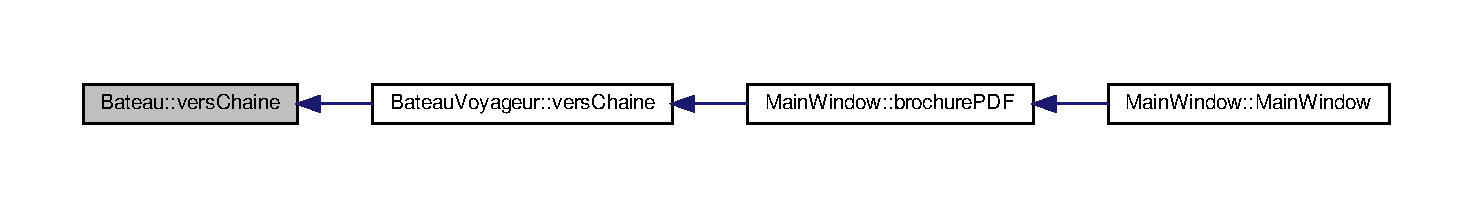
\includegraphics[width=350pt]{class_bateau_a392f6a45649a2a35186dfcd1ca58eddc_icgraph}
\end{center}
\end{figure}


\subsection{Documentation des données membres}
\mbox{\Hypertarget{class_bateau_acf710114558ee740be62211df06133e1}\label{class_bateau_acf710114558ee740be62211df06133e1}} 
\index{Bateau@{Bateau}!id\+Bat@{id\+Bat}}
\index{id\+Bat@{id\+Bat}!Bateau@{Bateau}}
\subsubsection{\texorpdfstring{id\+Bat}{idBat}}
{\footnotesize\ttfamily Q\+String Bateau\+::id\+Bat\hspace{0.3cm}{\ttfamily [private]}}



Définition à la ligne 18 du fichier bateau.\+h.

\mbox{\Hypertarget{class_bateau_ace3ced3b9bb6506a913645230b85022c}\label{class_bateau_ace3ced3b9bb6506a913645230b85022c}} 
\index{Bateau@{Bateau}!largeur\+Bat@{largeur\+Bat}}
\index{largeur\+Bat@{largeur\+Bat}!Bateau@{Bateau}}
\subsubsection{\texorpdfstring{largeur\+Bat}{largeurBat}}
{\footnotesize\ttfamily float Bateau\+::largeur\+Bat\hspace{0.3cm}{\ttfamily [private]}}



Définition à la ligne 19 du fichier bateau.\+h.

\mbox{\Hypertarget{class_bateau_a6c1f8f9f5bb656fae6ce59bcfa6fe8aa}\label{class_bateau_a6c1f8f9f5bb656fae6ce59bcfa6fe8aa}} 
\index{Bateau@{Bateau}!longueur\+Bat@{longueur\+Bat}}
\index{longueur\+Bat@{longueur\+Bat}!Bateau@{Bateau}}
\subsubsection{\texorpdfstring{longueur\+Bat}{longueurBat}}
{\footnotesize\ttfamily float Bateau\+::longueur\+Bat\hspace{0.3cm}{\ttfamily [private]}}



Définition à la ligne 19 du fichier bateau.\+h.

\mbox{\Hypertarget{class_bateau_a2d01e3edfc60cb9111a5f4f11b2813b3}\label{class_bateau_a2d01e3edfc60cb9111a5f4f11b2813b3}} 
\index{Bateau@{Bateau}!nom\+Bat@{nom\+Bat}}
\index{nom\+Bat@{nom\+Bat}!Bateau@{Bateau}}
\subsubsection{\texorpdfstring{nom\+Bat}{nomBat}}
{\footnotesize\ttfamily Q\+String Bateau\+::nom\+Bat\hspace{0.3cm}{\ttfamily [private]}}



Définition à la ligne 18 du fichier bateau.\+h.



La documentation de cette classe a été générée à partir des fichiers suivants \+:\begin{DoxyCompactItemize}
\item 
\hyperlink{bateau_8h}{bateau.\+h}\item 
\hyperlink{bateau_8cpp}{bateau.\+cpp}\end{DoxyCompactItemize}

\hypertarget{class_bateau_voyageur}{}\section{Référence de la classe Bateau\+Voyageur}
\label{class_bateau_voyageur}\index{Bateau\+Voyageur@{Bateau\+Voyageur}}


La classe \hyperlink{class_bateau_voyageur}{Bateau\+Voyageur} C\textquotesingle{}est une dépendance de la classe \hyperlink{class_passerelle}{Passerelle} Chaque bateau voyageur dispose de 3 propriétés.  




{\ttfamily \#include $<$bateauvoyageur.\+h$>$}



Graphe d\textquotesingle{}héritage de Bateau\+Voyageur\+:\nopagebreak
\begin{figure}[H]
\begin{center}
\leavevmode
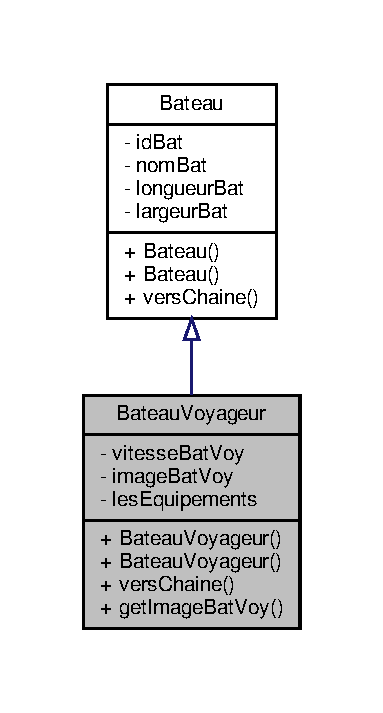
\includegraphics[width=184pt]{class_bateau_voyageur__inherit__graph}
\end{center}
\end{figure}


Graphe de collaboration de Bateau\+Voyageur\+:\nopagebreak
\begin{figure}[H]
\begin{center}
\leavevmode
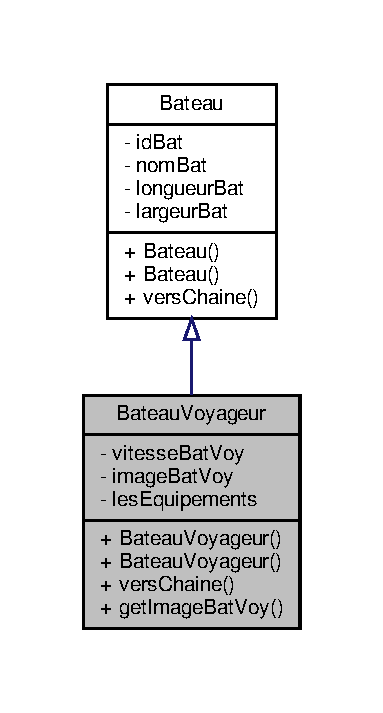
\includegraphics[width=184pt]{class_bateau_voyageur__coll__graph}
\end{center}
\end{figure}
\subsection*{Fonctions membres publiques}
\begin{DoxyCompactItemize}
\item 
\hyperlink{class_bateau_voyageur_ab2351c630bf3661b8273c66017c1ed72}{Bateau\+Voyageur} (Q\+String un\+Id, Q\+String un\+Nom, float une\+Longueur, float une\+Largeur, float une\+Vitesse, Q\+String une\+Image, Q\+Vector$<$ \hyperlink{class_equipement}{Equipement} $>$ une\+Coll\+Equip)
\begin{DoxyCompactList}\small\item\em \hyperlink{class_bateau_voyageur_ab2351c630bf3661b8273c66017c1ed72}{Bateau\+Voyageur\+::\+Bateau\+Voyageur} Constructeur de la classe \hyperlink{class_bateau_voyageur}{Bateau\+Voyageur} qui permet de renseigner les propriétés privées du \hyperlink{class_bateau_voyageur}{Bateau\+Voyageur} ainsi que celles du \hyperlink{class_bateau}{Bateau} avec les valeurs passées en paramètres Le constructeur de \hyperlink{class_bateau_voyageur}{Bateau\+Voyageur} appelle le constructeur de \hyperlink{class_bateau}{Bateau}. \end{DoxyCompactList}\item 
\hyperlink{class_bateau_voyageur_ac327b0101a2586190a3afcd639f146cc}{Bateau\+Voyageur} ()
\begin{DoxyCompactList}\small\item\em \hyperlink{class_bateau_voyageur_ab2351c630bf3661b8273c66017c1ed72}{Bateau\+Voyageur\+::\+Bateau\+Voyageur} Constructeur vide de la classe \hyperlink{class_bateau_voyageur}{Bateau\+Voyageur} nécessaire car il y a des vecteurs de \hyperlink{class_bateau_voyageur}{Bateau\+Voyageur}. \end{DoxyCompactList}\item 
Q\+String \hyperlink{class_bateau_voyageur_a3fa14cf7db3a1a35457f1e0450d7e8b2}{vers\+Chaine} ()
\begin{DoxyCompactList}\small\item\em \hyperlink{class_bateau_voyageur_a3fa14cf7db3a1a35457f1e0450d7e8b2}{Bateau\+Voyageur\+::vers\+Chaine} Méthode publique qui renvoie la chaîne de caractère utilisée pour décrire le bateau Cette méthode utilise la méthode \hyperlink{class_bateau_a392f6a45649a2a35186dfcd1ca58eddc}{Bateau\+::vers\+Chaine()}~\newline
Exemple \+:~\newline
Nom du bateau \+: Queen Mary~\newline
Longueur \+: 14.\+5 mètres~\newline
Largeur \+: 8.\+2 mètres~\newline
Vitesse \+: 21 noeuds~\newline
Liste des équipements du bateau \+:~\newline
-\/ Accès Handicapé~\newline
-\/ Bar. \end{DoxyCompactList}\item 
Q\+String \hyperlink{class_bateau_voyageur_a3154786b2f572d0c2a2ac975757295eb}{get\+Image\+Bat\+Voy} ()
\begin{DoxyCompactList}\small\item\em \hyperlink{class_bateau_voyageur_a3154786b2f572d0c2a2ac975757295eb}{Bateau\+Voyageur\+::get\+Image\+Bat\+Voy} Méthode publique qui renvoie le chemin qui permet d\textquotesingle{}atteindre l\textquotesingle{}image du bateau. \end{DoxyCompactList}\end{DoxyCompactItemize}
\subsection*{Attributs privés}
\begin{DoxyCompactItemize}
\item 
float \hyperlink{class_bateau_voyageur_a245a2e10cb6264193306f728b0af04cb}{vitesse\+Bat\+Voy}
\item 
Q\+String \hyperlink{class_bateau_voyageur_aa00ee12fc973cf555a5b07cbdcf573a3}{image\+Bat\+Voy}
\item 
Q\+Vector$<$ \hyperlink{class_equipement}{Equipement} $>$ \hyperlink{class_bateau_voyageur_a570ffdd189b44025d2e8d88e5dcdb1e2}{les\+Equipements}
\end{DoxyCompactItemize}


\subsection{Description détaillée}
La classe \hyperlink{class_bateau_voyageur}{Bateau\+Voyageur} C\textquotesingle{}est une dépendance de la classe \hyperlink{class_passerelle}{Passerelle} Chaque bateau voyageur dispose de 3 propriétés. 

\begin{DoxyAuthor}{Auteur}
Louis Vraie 
\end{DoxyAuthor}
\begin{DoxyDate}{Date}
08/11/2021 
\end{DoxyDate}
\begin{DoxyVersion}{Version}
1.\+0 beta 1 
\end{DoxyVersion}
\begin{DoxyCopyright}{Copyright}
G\+NU Public License 
\end{DoxyCopyright}


Définition à la ligne 18 du fichier bateauvoyageur.\+h.



\subsection{Documentation des constructeurs et destructeur}
\mbox{\Hypertarget{class_bateau_voyageur_ab2351c630bf3661b8273c66017c1ed72}\label{class_bateau_voyageur_ab2351c630bf3661b8273c66017c1ed72}} 
\index{Bateau\+Voyageur@{Bateau\+Voyageur}!Bateau\+Voyageur@{Bateau\+Voyageur}}
\index{Bateau\+Voyageur@{Bateau\+Voyageur}!Bateau\+Voyageur@{Bateau\+Voyageur}}
\subsubsection{\texorpdfstring{Bateau\+Voyageur()}{BateauVoyageur()}\hspace{0.1cm}{\footnotesize\ttfamily [1/2]}}
{\footnotesize\ttfamily Bateau\+Voyageur\+::\+Bateau\+Voyageur (\begin{DoxyParamCaption}\item[{Q\+String}]{un\+Id,  }\item[{Q\+String}]{un\+Nom,  }\item[{float}]{une\+Longueur,  }\item[{float}]{une\+Largeur,  }\item[{float}]{une\+Vitesse,  }\item[{Q\+String}]{une\+Image,  }\item[{Q\+Vector$<$ \hyperlink{class_equipement}{Equipement} $>$}]{une\+Coll\+Equip }\end{DoxyParamCaption})}



\hyperlink{class_bateau_voyageur_ab2351c630bf3661b8273c66017c1ed72}{Bateau\+Voyageur\+::\+Bateau\+Voyageur} Constructeur de la classe \hyperlink{class_bateau_voyageur}{Bateau\+Voyageur} qui permet de renseigner les propriétés privées du \hyperlink{class_bateau_voyageur}{Bateau\+Voyageur} ainsi que celles du \hyperlink{class_bateau}{Bateau} avec les valeurs passées en paramètres Le constructeur de \hyperlink{class_bateau_voyageur}{Bateau\+Voyageur} appelle le constructeur de \hyperlink{class_bateau}{Bateau}. 


\begin{DoxyParams}{Paramètres}
{\em un\+Id} & Q\+String Identifiant du bateau \\
\hline
{\em un\+Nom} & Q\+String Nom du bateau \\
\hline
{\em une\+Longueur} & float Longueur du bateau exprimée en mètres \\
\hline
{\em une\+Largeur} & float Largeur du bateau exprimée en mètres \\
\hline
{\em une\+Vitesse} & float Vitesse de croisière du bateau exprimée en noeuds \\
\hline
{\em une\+Image} & Q\+String Chemin pour atteindre l\textquotesingle{}image du bateau \\
\hline
{\em une\+Coll\+Equip} & Q\+Vector$<$\+Equipement$>$ Liste des équipements présents sur le bateau \\
\hline
\end{DoxyParams}


Définition à la ligne 15 du fichier bateauvoyageur.\+cpp.

\mbox{\Hypertarget{class_bateau_voyageur_ac327b0101a2586190a3afcd639f146cc}\label{class_bateau_voyageur_ac327b0101a2586190a3afcd639f146cc}} 
\index{Bateau\+Voyageur@{Bateau\+Voyageur}!Bateau\+Voyageur@{Bateau\+Voyageur}}
\index{Bateau\+Voyageur@{Bateau\+Voyageur}!Bateau\+Voyageur@{Bateau\+Voyageur}}
\subsubsection{\texorpdfstring{Bateau\+Voyageur()}{BateauVoyageur()}\hspace{0.1cm}{\footnotesize\ttfamily [2/2]}}
{\footnotesize\ttfamily Bateau\+Voyageur\+::\+Bateau\+Voyageur (\begin{DoxyParamCaption}{ }\end{DoxyParamCaption})}



\hyperlink{class_bateau_voyageur_ab2351c630bf3661b8273c66017c1ed72}{Bateau\+Voyageur\+::\+Bateau\+Voyageur} Constructeur vide de la classe \hyperlink{class_bateau_voyageur}{Bateau\+Voyageur} nécessaire car il y a des vecteurs de \hyperlink{class_bateau_voyageur}{Bateau\+Voyageur}. 



Définition à la ligne 29 du fichier bateauvoyageur.\+cpp.



\subsection{Documentation des fonctions membres}
\mbox{\Hypertarget{class_bateau_voyageur_a3154786b2f572d0c2a2ac975757295eb}\label{class_bateau_voyageur_a3154786b2f572d0c2a2ac975757295eb}} 
\index{Bateau\+Voyageur@{Bateau\+Voyageur}!get\+Image\+Bat\+Voy@{get\+Image\+Bat\+Voy}}
\index{get\+Image\+Bat\+Voy@{get\+Image\+Bat\+Voy}!Bateau\+Voyageur@{Bateau\+Voyageur}}
\subsubsection{\texorpdfstring{get\+Image\+Bat\+Voy()}{getImageBatVoy()}}
{\footnotesize\ttfamily Q\+String Bateau\+Voyageur\+::get\+Image\+Bat\+Voy (\begin{DoxyParamCaption}{ }\end{DoxyParamCaption})}



\hyperlink{class_bateau_voyageur_a3154786b2f572d0c2a2ac975757295eb}{Bateau\+Voyageur\+::get\+Image\+Bat\+Voy} Méthode publique qui renvoie le chemin qui permet d\textquotesingle{}atteindre l\textquotesingle{}image du bateau. 

\begin{DoxyReturn}{Renvoie}
Q\+String Une chaîne de caractères qui renseigne le chemin d\textquotesingle{}accès de l\textquotesingle{}image du bateau 
\end{DoxyReturn}


Définition à la ligne 68 du fichier bateauvoyageur.\+cpp.

Voici le graphe des appelants de cette fonction \+:\nopagebreak
\begin{figure}[H]
\begin{center}
\leavevmode
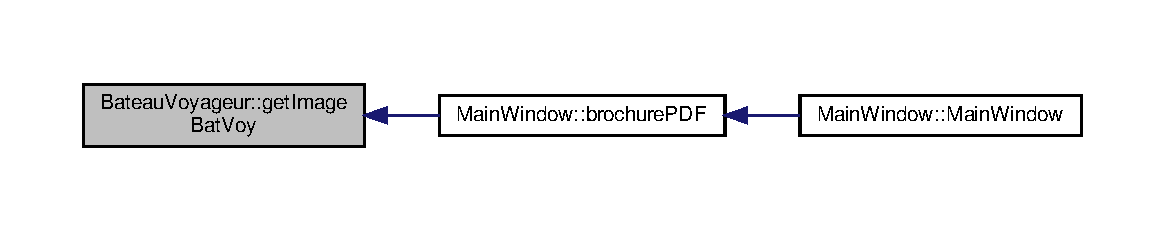
\includegraphics[width=350pt]{class_bateau_voyageur_a3154786b2f572d0c2a2ac975757295eb_icgraph}
\end{center}
\end{figure}
\mbox{\Hypertarget{class_bateau_voyageur_a3fa14cf7db3a1a35457f1e0450d7e8b2}\label{class_bateau_voyageur_a3fa14cf7db3a1a35457f1e0450d7e8b2}} 
\index{Bateau\+Voyageur@{Bateau\+Voyageur}!vers\+Chaine@{vers\+Chaine}}
\index{vers\+Chaine@{vers\+Chaine}!Bateau\+Voyageur@{Bateau\+Voyageur}}
\subsubsection{\texorpdfstring{vers\+Chaine()}{versChaine()}}
{\footnotesize\ttfamily Q\+String Bateau\+Voyageur\+::vers\+Chaine (\begin{DoxyParamCaption}{ }\end{DoxyParamCaption})}



\hyperlink{class_bateau_voyageur_a3fa14cf7db3a1a35457f1e0450d7e8b2}{Bateau\+Voyageur\+::vers\+Chaine} Méthode publique qui renvoie la chaîne de caractère utilisée pour décrire le bateau Cette méthode utilise la méthode \hyperlink{class_bateau_a392f6a45649a2a35186dfcd1ca58eddc}{Bateau\+::vers\+Chaine()}~\newline
Exemple \+:~\newline
Nom du bateau \+: Queen Mary~\newline
Longueur \+: 14.\+5 mètres~\newline
Largeur \+: 8.\+2 mètres~\newline
Vitesse \+: 21 noeuds~\newline
Liste des équipements du bateau \+:~\newline
-\/ Accès Handicapé~\newline
-\/ Bar. 

\begin{DoxyReturn}{Renvoie}
Q\+String Une chaîne de caractères sur plusieurs lignes qui renvoie toutes les informations associées à un bateau 
\end{DoxyReturn}


Définition à la ligne 48 du fichier bateauvoyageur.\+cpp.

Voici le graphe d\textquotesingle{}appel pour cette fonction \+:\nopagebreak
\begin{figure}[H]
\begin{center}
\leavevmode
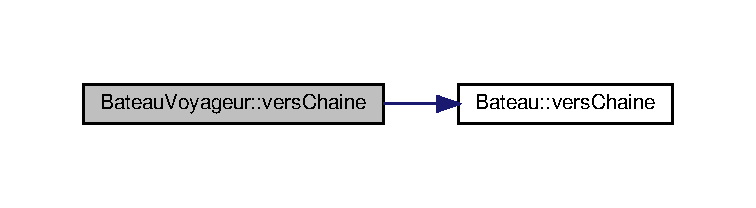
\includegraphics[width=350pt]{class_bateau_voyageur_a3fa14cf7db3a1a35457f1e0450d7e8b2_cgraph}
\end{center}
\end{figure}
Voici le graphe des appelants de cette fonction \+:\nopagebreak
\begin{figure}[H]
\begin{center}
\leavevmode
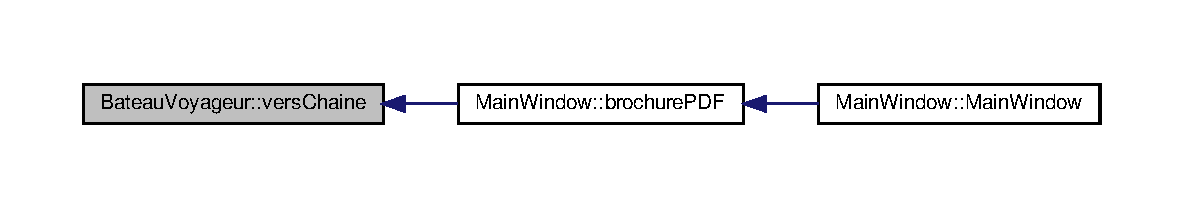
\includegraphics[width=350pt]{class_bateau_voyageur_a3fa14cf7db3a1a35457f1e0450d7e8b2_icgraph}
\end{center}
\end{figure}


\subsection{Documentation des données membres}
\mbox{\Hypertarget{class_bateau_voyageur_aa00ee12fc973cf555a5b07cbdcf573a3}\label{class_bateau_voyageur_aa00ee12fc973cf555a5b07cbdcf573a3}} 
\index{Bateau\+Voyageur@{Bateau\+Voyageur}!image\+Bat\+Voy@{image\+Bat\+Voy}}
\index{image\+Bat\+Voy@{image\+Bat\+Voy}!Bateau\+Voyageur@{Bateau\+Voyageur}}
\subsubsection{\texorpdfstring{image\+Bat\+Voy}{imageBatVoy}}
{\footnotesize\ttfamily Q\+String Bateau\+Voyageur\+::image\+Bat\+Voy\hspace{0.3cm}{\ttfamily [private]}}



Définition à la ligne 22 du fichier bateauvoyageur.\+h.

\mbox{\Hypertarget{class_bateau_voyageur_a570ffdd189b44025d2e8d88e5dcdb1e2}\label{class_bateau_voyageur_a570ffdd189b44025d2e8d88e5dcdb1e2}} 
\index{Bateau\+Voyageur@{Bateau\+Voyageur}!les\+Equipements@{les\+Equipements}}
\index{les\+Equipements@{les\+Equipements}!Bateau\+Voyageur@{Bateau\+Voyageur}}
\subsubsection{\texorpdfstring{les\+Equipements}{lesEquipements}}
{\footnotesize\ttfamily Q\+Vector$<$\hyperlink{class_equipement}{Equipement}$>$ Bateau\+Voyageur\+::les\+Equipements\hspace{0.3cm}{\ttfamily [private]}}



Définition à la ligne 23 du fichier bateauvoyageur.\+h.

\mbox{\Hypertarget{class_bateau_voyageur_a245a2e10cb6264193306f728b0af04cb}\label{class_bateau_voyageur_a245a2e10cb6264193306f728b0af04cb}} 
\index{Bateau\+Voyageur@{Bateau\+Voyageur}!vitesse\+Bat\+Voy@{vitesse\+Bat\+Voy}}
\index{vitesse\+Bat\+Voy@{vitesse\+Bat\+Voy}!Bateau\+Voyageur@{Bateau\+Voyageur}}
\subsubsection{\texorpdfstring{vitesse\+Bat\+Voy}{vitesseBatVoy}}
{\footnotesize\ttfamily float Bateau\+Voyageur\+::vitesse\+Bat\+Voy\hspace{0.3cm}{\ttfamily [private]}}



Définition à la ligne 21 du fichier bateauvoyageur.\+h.



La documentation de cette classe a été générée à partir des fichiers suivants \+:\begin{DoxyCompactItemize}
\item 
\hyperlink{bateauvoyageur_8h}{bateauvoyageur.\+h}\item 
\hyperlink{bateauvoyageur_8cpp}{bateauvoyageur.\+cpp}\end{DoxyCompactItemize}

\hypertarget{class_equipement}{}\section{Référence de la classe Equipement}
\label{class_equipement}\index{Equipement@{Equipement}}


La classe \hyperlink{class_equipement}{Equipement} C\textquotesingle{}est une dépendance de la classe \hyperlink{class_passerelle}{Passerelle} Chaque équipement possède 2 propriétés.  




{\ttfamily \#include $<$equipement.\+h$>$}



Graphe de collaboration de Equipement\+:\nopagebreak
\begin{figure}[H]
\begin{center}
\leavevmode
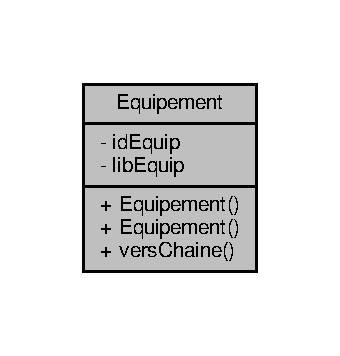
\includegraphics[width=163pt]{class_equipement__coll__graph}
\end{center}
\end{figure}
\subsection*{Fonctions membres publiques}
\begin{DoxyCompactItemize}
\item 
\hyperlink{class_equipement_a7017dfb537dadbaddac0d8006d96500b}{Equipement} (Q\+String son\+Id, Q\+String son\+Libelle)
\begin{DoxyCompactList}\small\item\em \hyperlink{class_equipement_a7017dfb537dadbaddac0d8006d96500b}{Equipement\+::\+Equipement} Constructeur de la classe \hyperlink{class_equipement}{Equipement} qui permet de remplir les propriétés privées de l\textquotesingle{}équipement avec les valeurs passées en paramètre. \end{DoxyCompactList}\item 
\hyperlink{class_equipement_a9057a4777d006cbac4c72d09a8d09407}{Equipement} ()
\begin{DoxyCompactList}\small\item\em \hyperlink{class_equipement_a7017dfb537dadbaddac0d8006d96500b}{Equipement\+::\+Equipement} Constructeur vide de la classe \hyperlink{class_equipement}{Equipement} nécessaire car il y a des vecteurs de \hyperlink{class_equipement}{Equipement}. \end{DoxyCompactList}\item 
Q\+String \hyperlink{class_equipement_a5e45c0b5524b353c77a23b618d73a1d0}{vers\+Chaine} ()
\begin{DoxyCompactList}\small\item\em \hyperlink{class_equipement_a5e45c0b5524b353c77a23b618d73a1d0}{Equipement\+::vers\+Chaine} Méthode publique qui renvoie la chaîne de caractère utilisée pour obtenir le libellé d\textquotesingle{}un équipement. \end{DoxyCompactList}\end{DoxyCompactItemize}
\subsection*{Attributs privés}
\begin{DoxyCompactItemize}
\item 
Q\+String \hyperlink{class_equipement_a140b7498ba59bdacb3f57a924b2853ad}{id\+Equip}
\item 
Q\+String \hyperlink{class_equipement_a69e0291bded262f34fe2ba57ad4cf99a}{lib\+Equip}
\end{DoxyCompactItemize}


\subsection{Description détaillée}
La classe \hyperlink{class_equipement}{Equipement} C\textquotesingle{}est une dépendance de la classe \hyperlink{class_passerelle}{Passerelle} Chaque équipement possède 2 propriétés. 

\begin{DoxyAuthor}{Auteur}
Louis Vraie 
\end{DoxyAuthor}
\begin{DoxyDate}{Date}
08/11/2021 
\end{DoxyDate}
\begin{DoxyVersion}{Version}
1.\+0 beta 1 
\end{DoxyVersion}
\begin{DoxyCopyright}{Copyright}
G\+NU Public License 
\end{DoxyCopyright}


Définition à la ligne 15 du fichier equipement.\+h.



\subsection{Documentation des constructeurs et destructeur}
\mbox{\Hypertarget{class_equipement_a7017dfb537dadbaddac0d8006d96500b}\label{class_equipement_a7017dfb537dadbaddac0d8006d96500b}} 
\index{Equipement@{Equipement}!Equipement@{Equipement}}
\index{Equipement@{Equipement}!Equipement@{Equipement}}
\subsubsection{\texorpdfstring{Equipement()}{Equipement()}\hspace{0.1cm}{\footnotesize\ttfamily [1/2]}}
{\footnotesize\ttfamily Equipement\+::\+Equipement (\begin{DoxyParamCaption}\item[{Q\+String}]{son\+Id,  }\item[{Q\+String}]{son\+Libelle }\end{DoxyParamCaption})}



\hyperlink{class_equipement_a7017dfb537dadbaddac0d8006d96500b}{Equipement\+::\+Equipement} Constructeur de la classe \hyperlink{class_equipement}{Equipement} qui permet de remplir les propriétés privées de l\textquotesingle{}équipement avec les valeurs passées en paramètre. 


\begin{DoxyParams}{Paramètres}
{\em son\+Id} & Q\+String Identifiant de l\textquotesingle{}équipement \\
\hline
{\em son\+Libelle} & Q\+String Libelle de l\textquotesingle{}équipement \\
\hline
\end{DoxyParams}


Définition à la ligne 8 du fichier equipement.\+cpp.

\mbox{\Hypertarget{class_equipement_a9057a4777d006cbac4c72d09a8d09407}\label{class_equipement_a9057a4777d006cbac4c72d09a8d09407}} 
\index{Equipement@{Equipement}!Equipement@{Equipement}}
\index{Equipement@{Equipement}!Equipement@{Equipement}}
\subsubsection{\texorpdfstring{Equipement()}{Equipement()}\hspace{0.1cm}{\footnotesize\ttfamily [2/2]}}
{\footnotesize\ttfamily Equipement\+::\+Equipement (\begin{DoxyParamCaption}{ }\end{DoxyParamCaption})}



\hyperlink{class_equipement_a7017dfb537dadbaddac0d8006d96500b}{Equipement\+::\+Equipement} Constructeur vide de la classe \hyperlink{class_equipement}{Equipement} nécessaire car il y a des vecteurs de \hyperlink{class_equipement}{Equipement}. 



Définition à la ligne 18 du fichier equipement.\+cpp.



\subsection{Documentation des fonctions membres}
\mbox{\Hypertarget{class_equipement_a5e45c0b5524b353c77a23b618d73a1d0}\label{class_equipement_a5e45c0b5524b353c77a23b618d73a1d0}} 
\index{Equipement@{Equipement}!vers\+Chaine@{vers\+Chaine}}
\index{vers\+Chaine@{vers\+Chaine}!Equipement@{Equipement}}
\subsubsection{\texorpdfstring{vers\+Chaine()}{versChaine()}}
{\footnotesize\ttfamily Q\+String Equipement\+::vers\+Chaine (\begin{DoxyParamCaption}{ }\end{DoxyParamCaption})}



\hyperlink{class_equipement_a5e45c0b5524b353c77a23b618d73a1d0}{Equipement\+::vers\+Chaine} Méthode publique qui renvoie la chaîne de caractère utilisée pour obtenir le libellé d\textquotesingle{}un équipement. 

\begin{DoxyReturn}{Renvoie}
Q\+String Une chaîne de caractères qui correspont au libellé de l\textquotesingle{}équipement 
\end{DoxyReturn}


Définition à la ligne 28 du fichier equipement.\+cpp.



\subsection{Documentation des données membres}
\mbox{\Hypertarget{class_equipement_a140b7498ba59bdacb3f57a924b2853ad}\label{class_equipement_a140b7498ba59bdacb3f57a924b2853ad}} 
\index{Equipement@{Equipement}!id\+Equip@{id\+Equip}}
\index{id\+Equip@{id\+Equip}!Equipement@{Equipement}}
\subsubsection{\texorpdfstring{id\+Equip}{idEquip}}
{\footnotesize\ttfamily Q\+String Equipement\+::id\+Equip\hspace{0.3cm}{\ttfamily [private]}}



Définition à la ligne 18 du fichier equipement.\+h.

\mbox{\Hypertarget{class_equipement_a69e0291bded262f34fe2ba57ad4cf99a}\label{class_equipement_a69e0291bded262f34fe2ba57ad4cf99a}} 
\index{Equipement@{Equipement}!lib\+Equip@{lib\+Equip}}
\index{lib\+Equip@{lib\+Equip}!Equipement@{Equipement}}
\subsubsection{\texorpdfstring{lib\+Equip}{libEquip}}
{\footnotesize\ttfamily Q\+String Equipement\+::lib\+Equip\hspace{0.3cm}{\ttfamily [private]}}



Définition à la ligne 18 du fichier equipement.\+h.



La documentation de cette classe a été générée à partir des fichiers suivants \+:\begin{DoxyCompactItemize}
\item 
\hyperlink{equipement_8h}{equipement.\+h}\item 
\hyperlink{equipement_8cpp}{equipement.\+cpp}\end{DoxyCompactItemize}

\hypertarget{class_jeu_enregistrement}{}\section{Référence de la classe Jeu\+Enregistrement}
\label{class_jeu_enregistrement}\index{Jeu\+Enregistrement@{Jeu\+Enregistrement}}


La classe \hyperlink{class_jeu_enregistrement}{Jeu\+Enregistrement} Elle hérite de la classe Q\+Sql\+Query Elle permet de manipuler un jeu de données.  




{\ttfamily \#include $<$jeuenregistrement.\+h$>$}



Graphe d\textquotesingle{}héritage de Jeu\+Enregistrement\+:\nopagebreak
\begin{figure}[H]
\begin{center}
\leavevmode
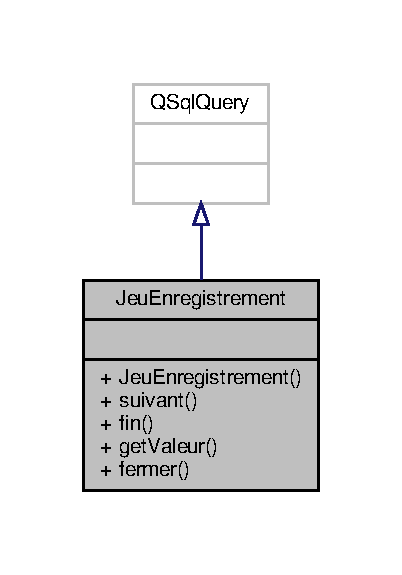
\includegraphics[width=193pt]{class_jeu_enregistrement__inherit__graph}
\end{center}
\end{figure}


Graphe de collaboration de Jeu\+Enregistrement\+:\nopagebreak
\begin{figure}[H]
\begin{center}
\leavevmode
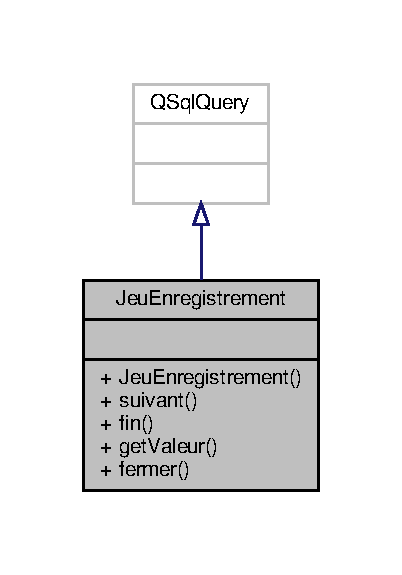
\includegraphics[width=193pt]{class_jeu_enregistrement__coll__graph}
\end{center}
\end{figure}
\subsection*{Fonctions membres publiques}
\begin{DoxyCompactItemize}
\item 
\hyperlink{class_jeu_enregistrement_ab7f4141f74961ae1d5060c6d19fae366}{Jeu\+Enregistrement} (Q\+String chaine\+Sql)
\begin{DoxyCompactList}\small\item\em \hyperlink{class_jeu_enregistrement_ab7f4141f74961ae1d5060c6d19fae366}{Jeu\+Enregistrement\+::\+Jeu\+Enregistrement} Constructeur de la classe \hyperlink{class_jeu_enregistrement}{Jeu\+Enregistrement} qui permet de lire un jeu d\textquotesingle{}enregistrement et de renseigner le paramètre de la classe Q\+Sql\+Query avec la chaîne S\+QL passées en paramètre Le constructeur de \hyperlink{class_jeu_enregistrement}{Jeu\+Enregistrement} appelle le constructeur de Q\+Sql\+Query. \end{DoxyCompactList}\item 
void \hyperlink{class_jeu_enregistrement_a4ac6b1c725cbb52f5320c514b7d65b71}{suivant} ()
\begin{DoxyCompactList}\small\item\em \hyperlink{class_jeu_enregistrement_a4ac6b1c725cbb52f5320c514b7d65b71}{Jeu\+Enregistrement\+::suivant} Méthode publique qui permet de passer à l\textquotesingle{}enregistrement suivant. \end{DoxyCompactList}\item 
bool \hyperlink{class_jeu_enregistrement_af8d23fbc407926e8578986a3e950bdd9}{fin} ()
\begin{DoxyCompactList}\small\item\em \hyperlink{class_jeu_enregistrement_af8d23fbc407926e8578986a3e950bdd9}{Jeu\+Enregistrement\+::fin} Méthode publique qui renvoie un booléen pour savoir si la fin du jeu d\textquotesingle{}enregistrement est atteint. \end{DoxyCompactList}\item 
Q\+Variant \hyperlink{class_jeu_enregistrement_aa19979b7af9747ae05e8e40f7747bbed}{get\+Valeur} (Q\+String nom\+Champ)
\begin{DoxyCompactList}\small\item\em \hyperlink{class_jeu_enregistrement_aa19979b7af9747ae05e8e40f7747bbed}{Jeu\+Enregistrement\+::get\+Valeur} Méthode publique qui renvoie la valeur du champ passé en paramètre. \end{DoxyCompactList}\item 
void \hyperlink{class_jeu_enregistrement_a25a6ae0b1b810abaeef0acb9876ecbaf}{fermer} ()
\begin{DoxyCompactList}\small\item\em \hyperlink{class_jeu_enregistrement_a25a6ae0b1b810abaeef0acb9876ecbaf}{Jeu\+Enregistrement\+::fermer} Méthode publique qui permet de marquer la fermeture de la requête. \end{DoxyCompactList}\end{DoxyCompactItemize}


\subsection{Description détaillée}
La classe \hyperlink{class_jeu_enregistrement}{Jeu\+Enregistrement} Elle hérite de la classe Q\+Sql\+Query Elle permet de manipuler un jeu de données. 

\begin{DoxyAuthor}{Auteur}
Louis Vraie 
\end{DoxyAuthor}
\begin{DoxyDate}{Date}
08/11/2021 
\end{DoxyDate}
\begin{DoxyVersion}{Version}
1.\+0 beta 1 
\end{DoxyVersion}
\begin{DoxyCopyright}{Copyright}
G\+NU Public License 
\end{DoxyCopyright}


Définition à la ligne 17 du fichier jeuenregistrement.\+h.



\subsection{Documentation des constructeurs et destructeur}
\mbox{\Hypertarget{class_jeu_enregistrement_ab7f4141f74961ae1d5060c6d19fae366}\label{class_jeu_enregistrement_ab7f4141f74961ae1d5060c6d19fae366}} 
\index{Jeu\+Enregistrement@{Jeu\+Enregistrement}!Jeu\+Enregistrement@{Jeu\+Enregistrement}}
\index{Jeu\+Enregistrement@{Jeu\+Enregistrement}!Jeu\+Enregistrement@{Jeu\+Enregistrement}}
\subsubsection{\texorpdfstring{Jeu\+Enregistrement()}{JeuEnregistrement()}}
{\footnotesize\ttfamily Jeu\+Enregistrement\+::\+Jeu\+Enregistrement (\begin{DoxyParamCaption}\item[{Q\+String}]{chaine\+Sql }\end{DoxyParamCaption})}



\hyperlink{class_jeu_enregistrement_ab7f4141f74961ae1d5060c6d19fae366}{Jeu\+Enregistrement\+::\+Jeu\+Enregistrement} Constructeur de la classe \hyperlink{class_jeu_enregistrement}{Jeu\+Enregistrement} qui permet de lire un jeu d\textquotesingle{}enregistrement et de renseigner le paramètre de la classe Q\+Sql\+Query avec la chaîne S\+QL passées en paramètre Le constructeur de \hyperlink{class_jeu_enregistrement}{Jeu\+Enregistrement} appelle le constructeur de Q\+Sql\+Query. 


\begin{DoxyParams}{Paramètres}
{\em chaine\+Sql} & Q\+String Requête S\+QL qui souhaite sélectionner des enregistrements dans une base de données \\
\hline
\end{DoxyParams}


Définition à la ligne 10 du fichier jeuenregistrement.\+cpp.



\subsection{Documentation des fonctions membres}
\mbox{\Hypertarget{class_jeu_enregistrement_a25a6ae0b1b810abaeef0acb9876ecbaf}\label{class_jeu_enregistrement_a25a6ae0b1b810abaeef0acb9876ecbaf}} 
\index{Jeu\+Enregistrement@{Jeu\+Enregistrement}!fermer@{fermer}}
\index{fermer@{fermer}!Jeu\+Enregistrement@{Jeu\+Enregistrement}}
\subsubsection{\texorpdfstring{fermer()}{fermer()}}
{\footnotesize\ttfamily void Jeu\+Enregistrement\+::fermer (\begin{DoxyParamCaption}{ }\end{DoxyParamCaption})}



\hyperlink{class_jeu_enregistrement_a25a6ae0b1b810abaeef0acb9876ecbaf}{Jeu\+Enregistrement\+::fermer} Méthode publique qui permet de marquer la fermeture de la requête. 



Définition à la ligne 50 du fichier jeuenregistrement.\+cpp.

\mbox{\Hypertarget{class_jeu_enregistrement_af8d23fbc407926e8578986a3e950bdd9}\label{class_jeu_enregistrement_af8d23fbc407926e8578986a3e950bdd9}} 
\index{Jeu\+Enregistrement@{Jeu\+Enregistrement}!fin@{fin}}
\index{fin@{fin}!Jeu\+Enregistrement@{Jeu\+Enregistrement}}
\subsubsection{\texorpdfstring{fin()}{fin()}}
{\footnotesize\ttfamily bool Jeu\+Enregistrement\+::fin (\begin{DoxyParamCaption}{ }\end{DoxyParamCaption})}



\hyperlink{class_jeu_enregistrement_af8d23fbc407926e8578986a3e950bdd9}{Jeu\+Enregistrement\+::fin} Méthode publique qui renvoie un booléen pour savoir si la fin du jeu d\textquotesingle{}enregistrement est atteint. 

\begin{DoxyReturn}{Renvoie}
bool Booléen qui permet de savoir si la fin du jeu d\textquotesingle{}enregistrement est atteint 
\end{DoxyReturn}


Définition à la ligne 30 du fichier jeuenregistrement.\+cpp.

Voici le graphe des appelants de cette fonction \+:\nopagebreak
\begin{figure}[H]
\begin{center}
\leavevmode
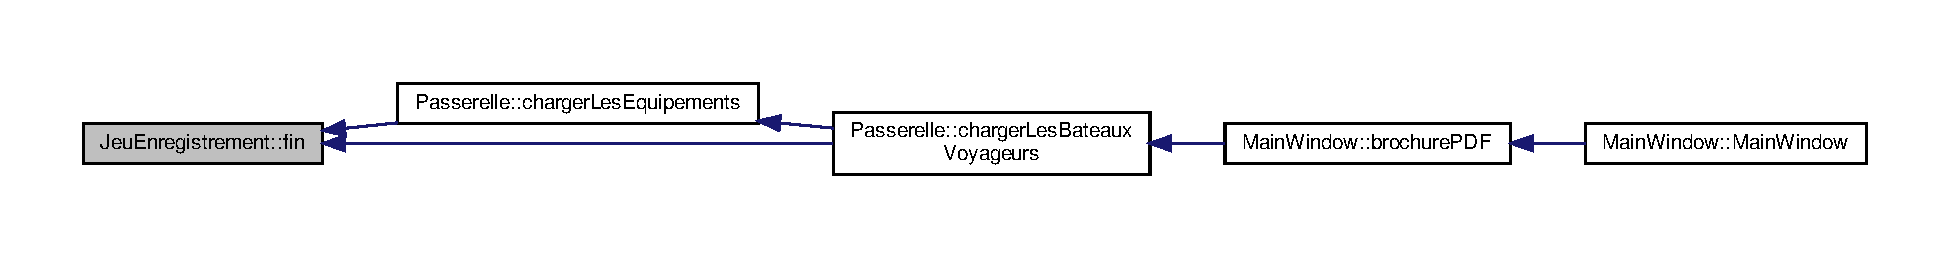
\includegraphics[width=350pt]{class_jeu_enregistrement_af8d23fbc407926e8578986a3e950bdd9_icgraph}
\end{center}
\end{figure}
\mbox{\Hypertarget{class_jeu_enregistrement_aa19979b7af9747ae05e8e40f7747bbed}\label{class_jeu_enregistrement_aa19979b7af9747ae05e8e40f7747bbed}} 
\index{Jeu\+Enregistrement@{Jeu\+Enregistrement}!get\+Valeur@{get\+Valeur}}
\index{get\+Valeur@{get\+Valeur}!Jeu\+Enregistrement@{Jeu\+Enregistrement}}
\subsubsection{\texorpdfstring{get\+Valeur()}{getValeur()}}
{\footnotesize\ttfamily Q\+Variant Jeu\+Enregistrement\+::get\+Valeur (\begin{DoxyParamCaption}\item[{Q\+String}]{nom\+Champ }\end{DoxyParamCaption})}



\hyperlink{class_jeu_enregistrement_aa19979b7af9747ae05e8e40f7747bbed}{Jeu\+Enregistrement\+::get\+Valeur} Méthode publique qui renvoie la valeur du champ passé en paramètre. 


\begin{DoxyParams}{Paramètres}
{\em nom\+Champ} & Q\+String Nom du champs à récupérer dans l\textquotesingle{}enregistrement courant \\
\hline
\end{DoxyParams}
\begin{DoxyReturn}{Renvoie}
Q\+Variant Variable non typé qui possède la valeur courante du champ donné en paramètre 
\end{DoxyReturn}


Définition à la ligne 41 du fichier jeuenregistrement.\+cpp.

Voici le graphe des appelants de cette fonction \+:\nopagebreak
\begin{figure}[H]
\begin{center}
\leavevmode
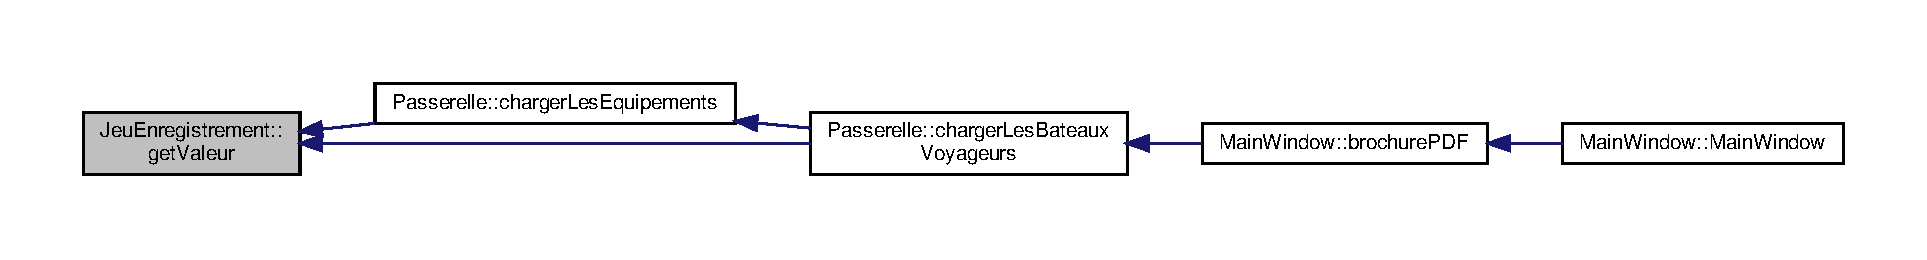
\includegraphics[width=350pt]{class_jeu_enregistrement_aa19979b7af9747ae05e8e40f7747bbed_icgraph}
\end{center}
\end{figure}
\mbox{\Hypertarget{class_jeu_enregistrement_a4ac6b1c725cbb52f5320c514b7d65b71}\label{class_jeu_enregistrement_a4ac6b1c725cbb52f5320c514b7d65b71}} 
\index{Jeu\+Enregistrement@{Jeu\+Enregistrement}!suivant@{suivant}}
\index{suivant@{suivant}!Jeu\+Enregistrement@{Jeu\+Enregistrement}}
\subsubsection{\texorpdfstring{suivant()}{suivant()}}
{\footnotesize\ttfamily void Jeu\+Enregistrement\+::suivant (\begin{DoxyParamCaption}{ }\end{DoxyParamCaption})}



\hyperlink{class_jeu_enregistrement_a4ac6b1c725cbb52f5320c514b7d65b71}{Jeu\+Enregistrement\+::suivant} Méthode publique qui permet de passer à l\textquotesingle{}enregistrement suivant. 



Définition à la ligne 20 du fichier jeuenregistrement.\+cpp.

Voici le graphe des appelants de cette fonction \+:\nopagebreak
\begin{figure}[H]
\begin{center}
\leavevmode
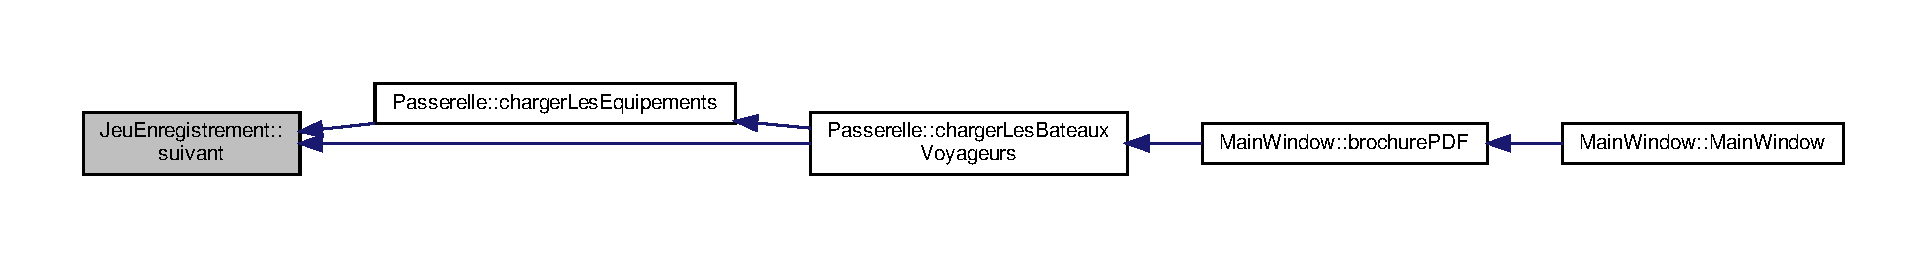
\includegraphics[width=350pt]{class_jeu_enregistrement_a4ac6b1c725cbb52f5320c514b7d65b71_icgraph}
\end{center}
\end{figure}


La documentation de cette classe a été générée à partir des fichiers suivants \+:\begin{DoxyCompactItemize}
\item 
\hyperlink{jeuenregistrement_8h}{jeuenregistrement.\+h}\item 
\hyperlink{jeuenregistrement_8cpp}{jeuenregistrement.\+cpp}\end{DoxyCompactItemize}

\hypertarget{class_main_window}{}\section{Référence de la classe Main\+Window}
\label{class_main_window}\index{Main\+Window@{Main\+Window}}


La classe \hyperlink{class_main_window}{Main\+Window} Elle hérite de la classe Q\+Main\+Window Elle permet de créer la fenêtre de l\textquotesingle{}application.  




{\ttfamily \#include $<$mainwindow.\+h$>$}



Graphe d\textquotesingle{}héritage de Main\+Window\+:\nopagebreak
\begin{figure}[H]
\begin{center}
\leavevmode
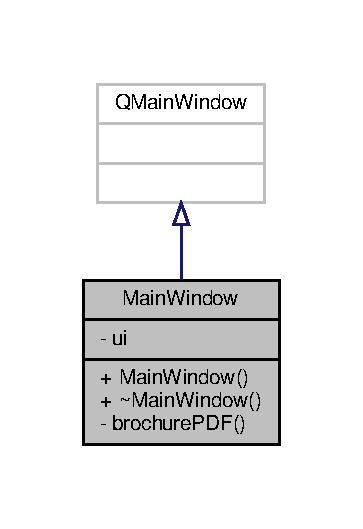
\includegraphics[width=174pt]{class_main_window__inherit__graph}
\end{center}
\end{figure}


Graphe de collaboration de Main\+Window\+:\nopagebreak
\begin{figure}[H]
\begin{center}
\leavevmode
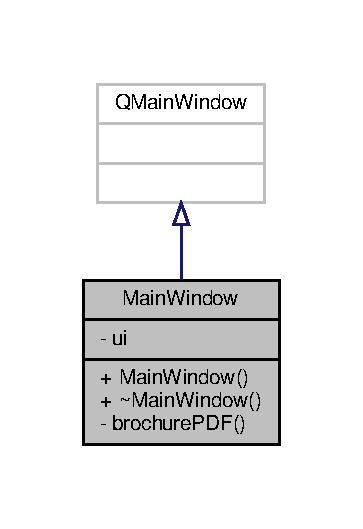
\includegraphics[width=174pt]{class_main_window__coll__graph}
\end{center}
\end{figure}
\subsection*{Fonctions membres publiques}
\begin{DoxyCompactItemize}
\item 
\hyperlink{class_main_window_a996c5a2b6f77944776856f08ec30858d}{Main\+Window} (Q\+Widget $\ast$parent=nullptr)
\begin{DoxyCompactList}\small\item\em \hyperlink{class_main_window_a996c5a2b6f77944776856f08ec30858d}{Main\+Window\+::\+Main\+Window} Constructeur de la classe \hyperlink{class_main_window}{Main\+Window} qui permet de créer l\textquotesingle{}application. \end{DoxyCompactList}\item 
\hyperlink{class_main_window_ae98d00a93bc118200eeef9f9bba1dba7}{$\sim$\+Main\+Window} ()
\begin{DoxyCompactList}\small\item\em \hyperlink{class_main_window_ae98d00a93bc118200eeef9f9bba1dba7}{Main\+Window\+::$\sim$\+Main\+Window} Destructeur de la classe \hyperlink{class_main_window}{Main\+Window} qui permet de détruire et donc fermer l\textquotesingle{}application. \end{DoxyCompactList}\end{DoxyCompactItemize}
\subsection*{Fonctions membres privées}
\begin{DoxyCompactItemize}
\item 
void \hyperlink{class_main_window_a6db0e3a1a7ce60c36d151d1ae618f16c}{brochure\+P\+DF} ()
\begin{DoxyCompactList}\small\item\em \hyperlink{class_main_window_a6db0e3a1a7ce60c36d151d1ae618f16c}{Main\+Window\+::brochure\+P\+DF} Méthode privée qui permet de créer une brochure \hyperlink{class_p_d_f}{P\+DF} des Bateaux\+Voyageur dans l\textquotesingle{}application. \end{DoxyCompactList}\end{DoxyCompactItemize}
\subsection*{Attributs privés}
\begin{DoxyCompactItemize}
\item 
Ui\+::\+Main\+Window $\ast$ \hyperlink{class_main_window_a35466a70ed47252a0191168126a352a5}{ui}
\end{DoxyCompactItemize}


\subsection{Description détaillée}
La classe \hyperlink{class_main_window}{Main\+Window} Elle hérite de la classe Q\+Main\+Window Elle permet de créer la fenêtre de l\textquotesingle{}application. 

Définition à la ligne 22 du fichier mainwindow.\+h.



\subsection{Documentation des constructeurs et destructeur}
\mbox{\Hypertarget{class_main_window_a996c5a2b6f77944776856f08ec30858d}\label{class_main_window_a996c5a2b6f77944776856f08ec30858d}} 
\index{Main\+Window@{Main\+Window}!Main\+Window@{Main\+Window}}
\index{Main\+Window@{Main\+Window}!Main\+Window@{Main\+Window}}
\subsubsection{\texorpdfstring{Main\+Window()}{MainWindow()}}
{\footnotesize\ttfamily Main\+Window\+::\+Main\+Window (\begin{DoxyParamCaption}\item[{Q\+Widget $\ast$}]{parent = {\ttfamily nullptr} }\end{DoxyParamCaption})\hspace{0.3cm}{\ttfamily [explicit]}}



\hyperlink{class_main_window_a996c5a2b6f77944776856f08ec30858d}{Main\+Window\+::\+Main\+Window} Constructeur de la classe \hyperlink{class_main_window}{Main\+Window} qui permet de créer l\textquotesingle{}application. 


\begin{DoxyParams}{Paramètres}
{\em parent} & Q\+Widget \\
\hline
\end{DoxyParams}


Définition à la ligne 12 du fichier mainwindow.\+cpp.

Voici le graphe d\textquotesingle{}appel pour cette fonction \+:\nopagebreak
\begin{figure}[H]
\begin{center}
\leavevmode
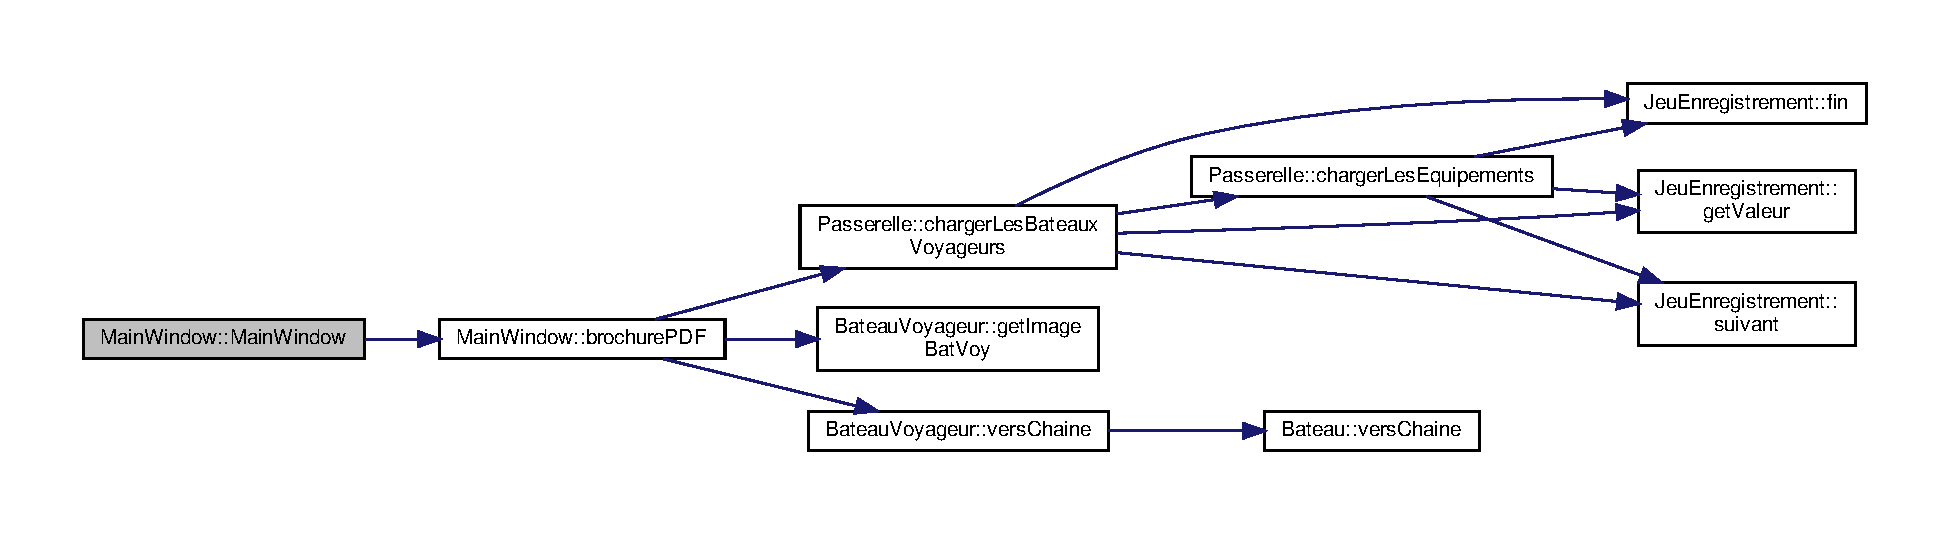
\includegraphics[width=350pt]{class_main_window_a996c5a2b6f77944776856f08ec30858d_cgraph}
\end{center}
\end{figure}
\mbox{\Hypertarget{class_main_window_ae98d00a93bc118200eeef9f9bba1dba7}\label{class_main_window_ae98d00a93bc118200eeef9f9bba1dba7}} 
\index{Main\+Window@{Main\+Window}!````~Main\+Window@{$\sim$\+Main\+Window}}
\index{````~Main\+Window@{$\sim$\+Main\+Window}!Main\+Window@{Main\+Window}}
\subsubsection{\texorpdfstring{$\sim$\+Main\+Window()}{~MainWindow()}}
{\footnotesize\ttfamily Main\+Window\+::$\sim$\+Main\+Window (\begin{DoxyParamCaption}{ }\end{DoxyParamCaption})}



\hyperlink{class_main_window_ae98d00a93bc118200eeef9f9bba1dba7}{Main\+Window\+::$\sim$\+Main\+Window} Destructeur de la classe \hyperlink{class_main_window}{Main\+Window} qui permet de détruire et donc fermer l\textquotesingle{}application. 



Définition à la ligne 25 du fichier mainwindow.\+cpp.



\subsection{Documentation des fonctions membres}
\mbox{\Hypertarget{class_main_window_a6db0e3a1a7ce60c36d151d1ae618f16c}\label{class_main_window_a6db0e3a1a7ce60c36d151d1ae618f16c}} 
\index{Main\+Window@{Main\+Window}!brochure\+P\+DF@{brochure\+P\+DF}}
\index{brochure\+P\+DF@{brochure\+P\+DF}!Main\+Window@{Main\+Window}}
\subsubsection{\texorpdfstring{brochure\+P\+D\+F()}{brochurePDF()}}
{\footnotesize\ttfamily void Main\+Window\+::brochure\+P\+DF (\begin{DoxyParamCaption}{ }\end{DoxyParamCaption})\hspace{0.3cm}{\ttfamily [private]}}



\hyperlink{class_main_window_a6db0e3a1a7ce60c36d151d1ae618f16c}{Main\+Window\+::brochure\+P\+DF} Méthode privée qui permet de créer une brochure \hyperlink{class_p_d_f}{P\+DF} des Bateaux\+Voyageur dans l\textquotesingle{}application. 



Définition à la ligne 34 du fichier mainwindow.\+cpp.

Voici le graphe d\textquotesingle{}appel pour cette fonction \+:\nopagebreak
\begin{figure}[H]
\begin{center}
\leavevmode
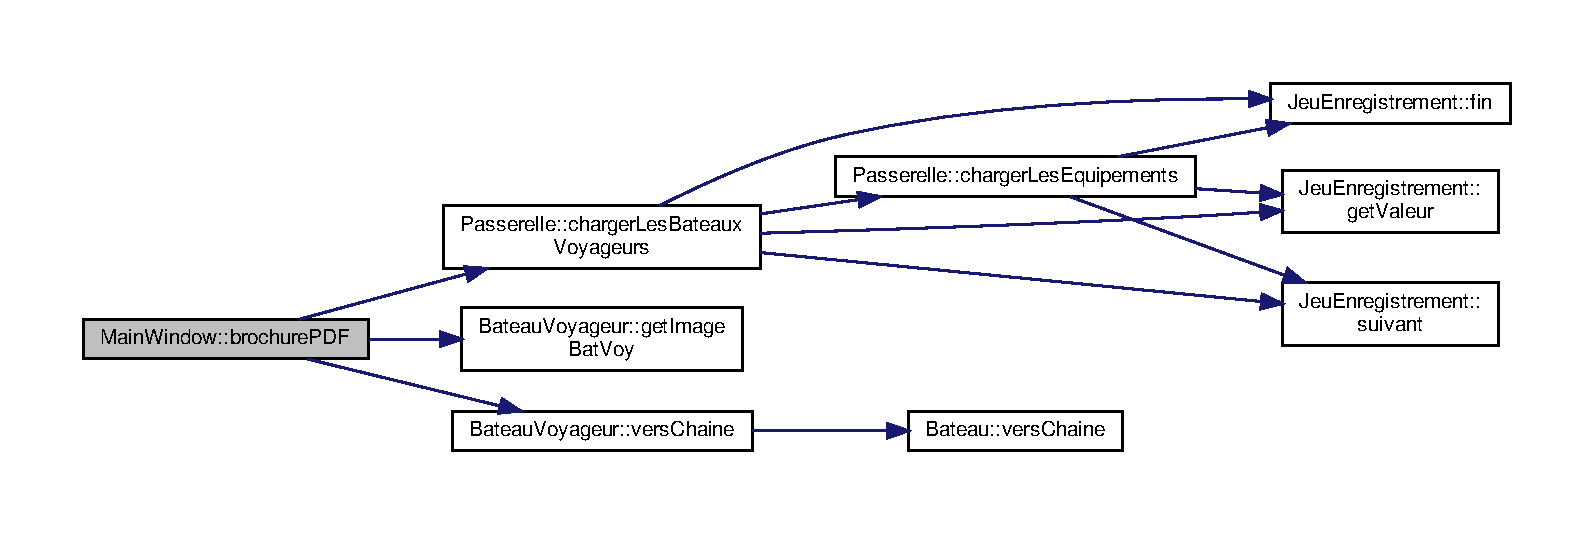
\includegraphics[width=350pt]{class_main_window_a6db0e3a1a7ce60c36d151d1ae618f16c_cgraph}
\end{center}
\end{figure}
Voici le graphe des appelants de cette fonction \+:\nopagebreak
\begin{figure}[H]
\begin{center}
\leavevmode
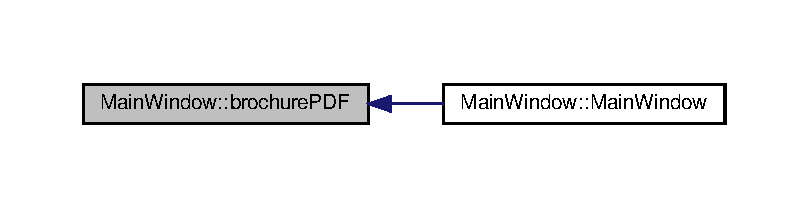
\includegraphics[width=350pt]{class_main_window_a6db0e3a1a7ce60c36d151d1ae618f16c_icgraph}
\end{center}
\end{figure}


\subsection{Documentation des données membres}
\mbox{\Hypertarget{class_main_window_a35466a70ed47252a0191168126a352a5}\label{class_main_window_a35466a70ed47252a0191168126a352a5}} 
\index{Main\+Window@{Main\+Window}!ui@{ui}}
\index{ui@{ui}!Main\+Window@{Main\+Window}}
\subsubsection{\texorpdfstring{ui}{ui}}
{\footnotesize\ttfamily Ui\+::\+Main\+Window$\ast$ Main\+Window\+::ui\hspace{0.3cm}{\ttfamily [private]}}



Définition à la ligne 31 du fichier mainwindow.\+h.



La documentation de cette classe a été générée à partir des fichiers suivants \+:\begin{DoxyCompactItemize}
\item 
\hyperlink{mainwindow_8h}{mainwindow.\+h}\item 
\hyperlink{mainwindow_8cpp}{mainwindow.\+cpp}\end{DoxyCompactItemize}

\hypertarget{class_passerelle}{}\section{Référence de la classe Passerelle}
\label{class_passerelle}\index{Passerelle@{Passerelle}}


La classe \hyperlink{class_passerelle}{Passerelle} Elle est dépendante des classes \hyperlink{class_bateau_voyageur}{Bateau\+Voyageur} et \hyperlink{class_equipement}{Equipement}.  




{\ttfamily \#include $<$passerelle.\+h$>$}



Graphe de collaboration de Passerelle\+:\nopagebreak
\begin{figure}[H]
\begin{center}
\leavevmode
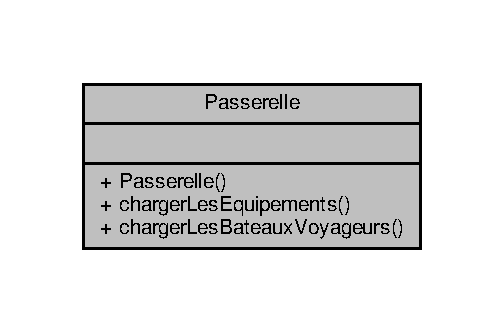
\includegraphics[width=242pt]{class_passerelle__coll__graph}
\end{center}
\end{figure}
\subsection*{Fonctions membres publiques}
\begin{DoxyCompactItemize}
\item 
\hyperlink{class_passerelle_ab70aa7f8273e11735416362091d6c5f4}{Passerelle} ()
\begin{DoxyCompactList}\small\item\em \hyperlink{class_passerelle_ab70aa7f8273e11735416362091d6c5f4}{Passerelle\+::\+Passerelle} Constructeur vide de la classe \hyperlink{class_passerelle}{Passerelle}. \end{DoxyCompactList}\end{DoxyCompactItemize}
\subsection*{Fonctions membres publiques statiques}
\begin{DoxyCompactItemize}
\item 
static Q\+Vector$<$ \hyperlink{class_equipement}{Equipement} $>$ \hyperlink{class_passerelle_a7388ba173e23ebf4ceb26d878e9503b3}{charger\+Les\+Equipements} (int un\+Id\+Bateau)
\begin{DoxyCompactList}\small\item\em \hyperlink{class_passerelle_a7388ba173e23ebf4ceb26d878e9503b3}{Passerelle\+::charger\+Les\+Equipements} Méthode statique publique qui permet de charger les différents équipements d\textquotesingle{}un bateau avec son identifiant passé en paramètre. \end{DoxyCompactList}\item 
static Q\+Vector$<$ \hyperlink{class_bateau_voyageur}{Bateau\+Voyageur} $>$ \hyperlink{class_passerelle_a9f8cdd9d52d668bb33a5380324fb9c51}{charger\+Les\+Bateaux\+Voyageurs} ()
\begin{DoxyCompactList}\small\item\em \hyperlink{class_passerelle_a9f8cdd9d52d668bb33a5380324fb9c51}{Passerelle\+::charger\+Les\+Bateaux\+Voyageurs} Méthode statique publique qui permet de charger les différentes informations de tous les bateaux voyageurs. \end{DoxyCompactList}\end{DoxyCompactItemize}


\subsection{Description détaillée}
La classe \hyperlink{class_passerelle}{Passerelle} Elle est dépendante des classes \hyperlink{class_bateau_voyageur}{Bateau\+Voyageur} et \hyperlink{class_equipement}{Equipement}. 

\begin{DoxyAuthor}{Auteur}
Louis Vraie 
\end{DoxyAuthor}
\begin{DoxyDate}{Date}
08/11/2021 
\end{DoxyDate}
\begin{DoxyVersion}{Version}
1.\+0 beta 1 
\end{DoxyVersion}
\begin{DoxyCopyright}{Copyright}
G\+NU Public License 
\end{DoxyCopyright}


Définition à la ligne 18 du fichier passerelle.\+h.



\subsection{Documentation des constructeurs et destructeur}
\mbox{\Hypertarget{class_passerelle_ab70aa7f8273e11735416362091d6c5f4}\label{class_passerelle_ab70aa7f8273e11735416362091d6c5f4}} 
\index{Passerelle@{Passerelle}!Passerelle@{Passerelle}}
\index{Passerelle@{Passerelle}!Passerelle@{Passerelle}}
\subsubsection{\texorpdfstring{Passerelle()}{Passerelle()}}
{\footnotesize\ttfamily Passerelle\+::\+Passerelle (\begin{DoxyParamCaption}{ }\end{DoxyParamCaption})}



\hyperlink{class_passerelle_ab70aa7f8273e11735416362091d6c5f4}{Passerelle\+::\+Passerelle} Constructeur vide de la classe \hyperlink{class_passerelle}{Passerelle}. 



Définition à la ligne 7 du fichier passerelle.\+cpp.



\subsection{Documentation des fonctions membres}
\mbox{\Hypertarget{class_passerelle_a9f8cdd9d52d668bb33a5380324fb9c51}\label{class_passerelle_a9f8cdd9d52d668bb33a5380324fb9c51}} 
\index{Passerelle@{Passerelle}!charger\+Les\+Bateaux\+Voyageurs@{charger\+Les\+Bateaux\+Voyageurs}}
\index{charger\+Les\+Bateaux\+Voyageurs@{charger\+Les\+Bateaux\+Voyageurs}!Passerelle@{Passerelle}}
\subsubsection{\texorpdfstring{charger\+Les\+Bateaux\+Voyageurs()}{chargerLesBateauxVoyageurs()}}
{\footnotesize\ttfamily Q\+Vector$<$ \hyperlink{class_bateau_voyageur}{Bateau\+Voyageur} $>$ Passerelle\+::charger\+Les\+Bateaux\+Voyageurs (\begin{DoxyParamCaption}{ }\end{DoxyParamCaption})\hspace{0.3cm}{\ttfamily [static]}}



\hyperlink{class_passerelle_a9f8cdd9d52d668bb33a5380324fb9c51}{Passerelle\+::charger\+Les\+Bateaux\+Voyageurs} Méthode statique publique qui permet de charger les différentes informations de tous les bateaux voyageurs. 

\begin{DoxyReturn}{Renvoie}
Q\+Vector$<$\+Bateau\+Voyageur$>$ Vecteur qui contient toutes les informations associées aux bateaux voyageurs (le numéro, le libellé, les détails techniques, l\textquotesingle{}image et les équipements) 
\end{DoxyReturn}


Définition à la ligne 45 du fichier passerelle.\+cpp.

Voici le graphe d\textquotesingle{}appel pour cette fonction \+:\nopagebreak
\begin{figure}[H]
\begin{center}
\leavevmode
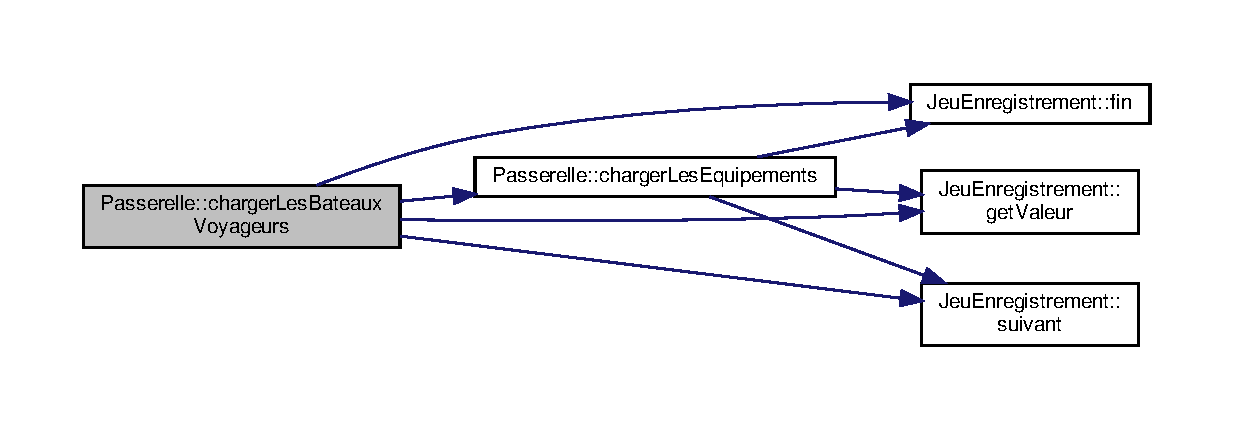
\includegraphics[width=350pt]{class_passerelle_a9f8cdd9d52d668bb33a5380324fb9c51_cgraph}
\end{center}
\end{figure}
Voici le graphe des appelants de cette fonction \+:\nopagebreak
\begin{figure}[H]
\begin{center}
\leavevmode
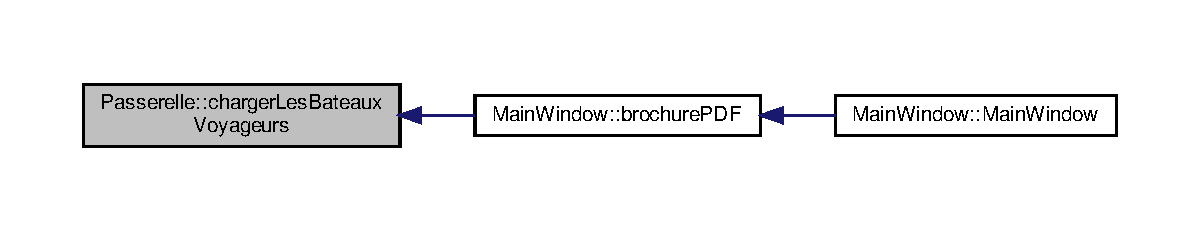
\includegraphics[width=350pt]{class_passerelle_a9f8cdd9d52d668bb33a5380324fb9c51_icgraph}
\end{center}
\end{figure}
\mbox{\Hypertarget{class_passerelle_a7388ba173e23ebf4ceb26d878e9503b3}\label{class_passerelle_a7388ba173e23ebf4ceb26d878e9503b3}} 
\index{Passerelle@{Passerelle}!charger\+Les\+Equipements@{charger\+Les\+Equipements}}
\index{charger\+Les\+Equipements@{charger\+Les\+Equipements}!Passerelle@{Passerelle}}
\subsubsection{\texorpdfstring{charger\+Les\+Equipements()}{chargerLesEquipements()}}
{\footnotesize\ttfamily Q\+Vector$<$ \hyperlink{class_equipement}{Equipement} $>$ Passerelle\+::charger\+Les\+Equipements (\begin{DoxyParamCaption}\item[{int}]{un\+Id\+Bateau }\end{DoxyParamCaption})\hspace{0.3cm}{\ttfamily [static]}}



\hyperlink{class_passerelle_a7388ba173e23ebf4ceb26d878e9503b3}{Passerelle\+::charger\+Les\+Equipements} Méthode statique publique qui permet de charger les différents équipements d\textquotesingle{}un bateau avec son identifiant passé en paramètre. 


\begin{DoxyParams}{Paramètres}
{\em un\+Id\+Bateau} & int Identifiant d\textquotesingle{}un bateau \\
\hline
\end{DoxyParams}
\begin{DoxyReturn}{Renvoie}
Q\+Vector$<$\+Equipement$>$ Vecteur qui contient tous les identifiants et les libellés des équipements d\textquotesingle{}un bateau 
\end{DoxyReturn}


Définition à la ligne 18 du fichier passerelle.\+cpp.

Voici le graphe d\textquotesingle{}appel pour cette fonction \+:\nopagebreak
\begin{figure}[H]
\begin{center}
\leavevmode
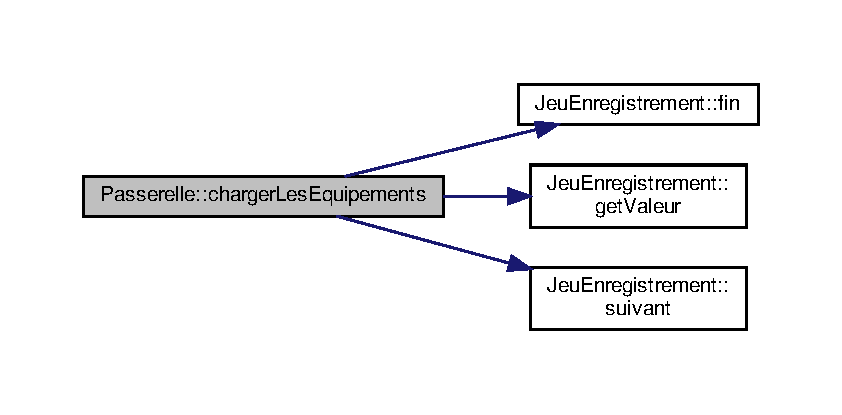
\includegraphics[width=350pt]{class_passerelle_a7388ba173e23ebf4ceb26d878e9503b3_cgraph}
\end{center}
\end{figure}
Voici le graphe des appelants de cette fonction \+:\nopagebreak
\begin{figure}[H]
\begin{center}
\leavevmode
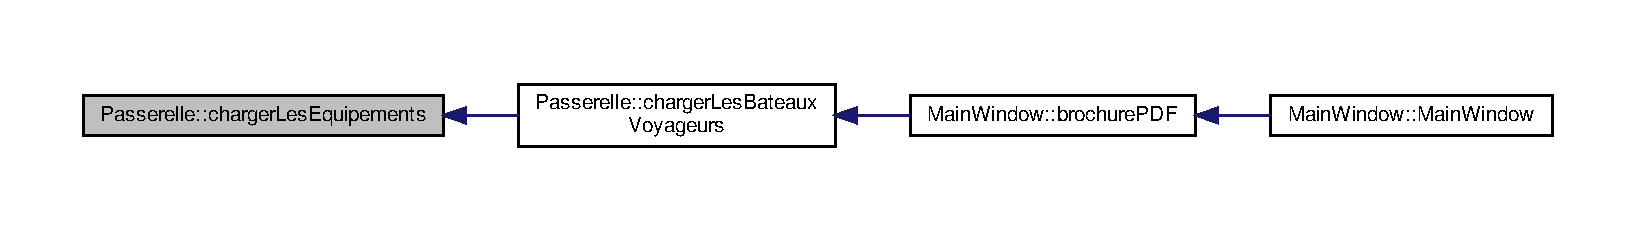
\includegraphics[width=350pt]{class_passerelle_a7388ba173e23ebf4ceb26d878e9503b3_icgraph}
\end{center}
\end{figure}


La documentation de cette classe a été générée à partir des fichiers suivants \+:\begin{DoxyCompactItemize}
\item 
\hyperlink{passerelle_8h}{passerelle.\+h}\item 
\hyperlink{passerelle_8cpp}{passerelle.\+cpp}\end{DoxyCompactItemize}

\hypertarget{class_p_d_f}{}\section{Référence de la classe P\+DF}
\label{class_p_d_f}\index{P\+DF@{P\+DF}}


La classe \hyperlink{class_p_d_f}{P\+DF} Elle hérite de la classe Q\+Text\+Browser Elle permet de générer un document \hyperlink{class_p_d_f}{P\+DF} Chaque pdf d\textquotesingle{}une propriété  




{\ttfamily \#include $<$pdf.\+h$>$}



Graphe d\textquotesingle{}héritage de P\+DF\+:\nopagebreak
\begin{figure}[H]
\begin{center}
\leavevmode
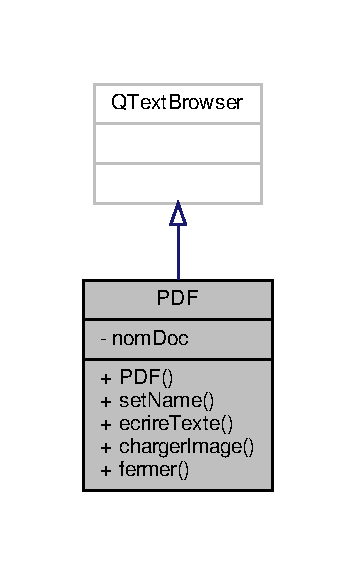
\includegraphics[width=171pt]{class_p_d_f__inherit__graph}
\end{center}
\end{figure}


Graphe de collaboration de P\+DF\+:\nopagebreak
\begin{figure}[H]
\begin{center}
\leavevmode
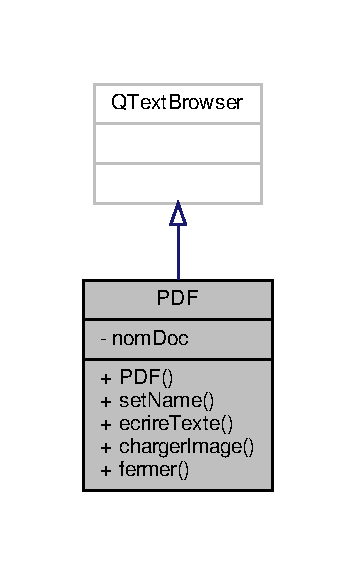
\includegraphics[width=171pt]{class_p_d_f__coll__graph}
\end{center}
\end{figure}
\subsection*{Fonctions membres publiques}
\begin{DoxyCompactItemize}
\item 
\hyperlink{class_p_d_f_af73fdd2d9d2d8aad204895ff5ffd35c4}{P\+DF} (Q\+Widget $\ast$parent)
\begin{DoxyCompactList}\small\item\em \hyperlink{class_p_d_f_af73fdd2d9d2d8aad204895ff5ffd35c4}{P\+D\+F\+::\+P\+DF} Constructeur vide de la classe \hyperlink{class_p_d_f}{P\+DF} qui permet de renseigner le paramètre de la classe Q\+Text\+Browser. \end{DoxyCompactList}\item 
void \hyperlink{class_p_d_f_a09ab186beccd7afa32dd947532a83e78}{set\+Name} (Q\+String nom\+Document)
\begin{DoxyCompactList}\small\item\em \hyperlink{class_p_d_f_a09ab186beccd7afa32dd947532a83e78}{P\+D\+F\+::set\+Name} Méthode publique qui permet de définir le nom du \hyperlink{class_p_d_f}{P\+DF}. \end{DoxyCompactList}\item 
void \hyperlink{class_p_d_f_a7bb38923f4141702b3772ec41213917f}{ecrire\+Texte} (Q\+String le\+Texte)
\begin{DoxyCompactList}\small\item\em \hyperlink{class_p_d_f_a7bb38923f4141702b3772ec41213917f}{P\+D\+F\+::ecrire\+Texte} Méthode publique qui permet d\textquotesingle{}ajouter le texte passé en paramètre au document \hyperlink{class_p_d_f}{P\+DF}. \end{DoxyCompactList}\item 
void \hyperlink{class_p_d_f_a3c7d97ad7f3c7a390272d05c7f95e832}{charger\+Image} (Q\+String chemin)
\begin{DoxyCompactList}\small\item\em \hyperlink{class_p_d_f_a3c7d97ad7f3c7a390272d05c7f95e832}{P\+D\+F\+::charger\+Image} Méthode publique qui permet d\textquotesingle{}ajouter le code H\+T\+ML qui permet d\textquotesingle{}afficher une image avec le chemin d\textquotesingle{}accès passé en paramètres. \end{DoxyCompactList}\item 
void \hyperlink{class_p_d_f_a96a1cc767274d19eedec45ff7aca6b7a}{fermer} ()
\begin{DoxyCompactList}\small\item\em \hyperlink{class_p_d_f_a96a1cc767274d19eedec45ff7aca6b7a}{P\+D\+F\+::fermer} Méthode publique qui permet de fermer le pdf en l\textquotesingle{}enregistrant et l\textquotesingle{}affichant. \end{DoxyCompactList}\end{DoxyCompactItemize}
\subsection*{Attributs privés}
\begin{DoxyCompactItemize}
\item 
Q\+String \hyperlink{class_p_d_f_ab62ed8b5ba6389035dd0aa0455ffd4f2}{nom\+Doc}
\end{DoxyCompactItemize}


\subsection{Description détaillée}
La classe \hyperlink{class_p_d_f}{P\+DF} Elle hérite de la classe Q\+Text\+Browser Elle permet de générer un document \hyperlink{class_p_d_f}{P\+DF} Chaque pdf d\textquotesingle{}une propriété 

\begin{DoxyAuthor}{Auteur}
Louis Vraie 
\end{DoxyAuthor}
\begin{DoxyDate}{Date}
08/11/2021 
\end{DoxyDate}
\begin{DoxyVersion}{Version}
1.\+0 beta 1 
\end{DoxyVersion}
\begin{DoxyCopyright}{Copyright}
G\+NU Public License 
\end{DoxyCopyright}


Définition à la ligne 20 du fichier pdf.\+h.



\subsection{Documentation des constructeurs et destructeur}
\mbox{\Hypertarget{class_p_d_f_af73fdd2d9d2d8aad204895ff5ffd35c4}\label{class_p_d_f_af73fdd2d9d2d8aad204895ff5ffd35c4}} 
\index{P\+DF@{P\+DF}!P\+DF@{P\+DF}}
\index{P\+DF@{P\+DF}!P\+DF@{P\+DF}}
\subsubsection{\texorpdfstring{P\+D\+F()}{PDF()}}
{\footnotesize\ttfamily P\+D\+F\+::\+P\+DF (\begin{DoxyParamCaption}\item[{Q\+Widget $\ast$}]{parent }\end{DoxyParamCaption})}



\hyperlink{class_p_d_f_af73fdd2d9d2d8aad204895ff5ffd35c4}{P\+D\+F\+::\+P\+DF} Constructeur vide de la classe \hyperlink{class_p_d_f}{P\+DF} qui permet de renseigner le paramètre de la classe Q\+Text\+Browser. 


\begin{DoxyParams}{Paramètres}
{\em parent} & Q\+Widget \\
\hline
\end{DoxyParams}


Définition à la ligne 8 du fichier pdf.\+cpp.



\subsection{Documentation des fonctions membres}
\mbox{\Hypertarget{class_p_d_f_a3c7d97ad7f3c7a390272d05c7f95e832}\label{class_p_d_f_a3c7d97ad7f3c7a390272d05c7f95e832}} 
\index{P\+DF@{P\+DF}!charger\+Image@{charger\+Image}}
\index{charger\+Image@{charger\+Image}!P\+DF@{P\+DF}}
\subsubsection{\texorpdfstring{charger\+Image()}{chargerImage()}}
{\footnotesize\ttfamily void P\+D\+F\+::charger\+Image (\begin{DoxyParamCaption}\item[{Q\+String}]{chemin }\end{DoxyParamCaption})}



\hyperlink{class_p_d_f_a3c7d97ad7f3c7a390272d05c7f95e832}{P\+D\+F\+::charger\+Image} Méthode publique qui permet d\textquotesingle{}ajouter le code H\+T\+ML qui permet d\textquotesingle{}afficher une image avec le chemin d\textquotesingle{}accès passé en paramètres. 


\begin{DoxyParams}{Paramètres}
{\em chemin} & Q\+String Chemin d\textquotesingle{}accès pour accéder à l\textquotesingle{}image \\
\hline
\end{DoxyParams}


Définition à la ligne 39 du fichier pdf.\+cpp.

\mbox{\Hypertarget{class_p_d_f_a7bb38923f4141702b3772ec41213917f}\label{class_p_d_f_a7bb38923f4141702b3772ec41213917f}} 
\index{P\+DF@{P\+DF}!ecrire\+Texte@{ecrire\+Texte}}
\index{ecrire\+Texte@{ecrire\+Texte}!P\+DF@{P\+DF}}
\subsubsection{\texorpdfstring{ecrire\+Texte()}{ecrireTexte()}}
{\footnotesize\ttfamily void P\+D\+F\+::ecrire\+Texte (\begin{DoxyParamCaption}\item[{Q\+String}]{le\+Texte }\end{DoxyParamCaption})}



\hyperlink{class_p_d_f_a7bb38923f4141702b3772ec41213917f}{P\+D\+F\+::ecrire\+Texte} Méthode publique qui permet d\textquotesingle{}ajouter le texte passé en paramètre au document \hyperlink{class_p_d_f}{P\+DF}. 


\begin{DoxyParams}{Paramètres}
{\em le\+Texte} & Q\+String \\
\hline
\end{DoxyParams}


Définition à la ligne 28 du fichier pdf.\+cpp.

\mbox{\Hypertarget{class_p_d_f_a96a1cc767274d19eedec45ff7aca6b7a}\label{class_p_d_f_a96a1cc767274d19eedec45ff7aca6b7a}} 
\index{P\+DF@{P\+DF}!fermer@{fermer}}
\index{fermer@{fermer}!P\+DF@{P\+DF}}
\subsubsection{\texorpdfstring{fermer()}{fermer()}}
{\footnotesize\ttfamily void P\+D\+F\+::fermer (\begin{DoxyParamCaption}{ }\end{DoxyParamCaption})}



\hyperlink{class_p_d_f_a96a1cc767274d19eedec45ff7aca6b7a}{P\+D\+F\+::fermer} Méthode publique qui permet de fermer le pdf en l\textquotesingle{}enregistrant et l\textquotesingle{}affichant. 



Définition à la ligne 49 du fichier pdf.\+cpp.

\mbox{\Hypertarget{class_p_d_f_a09ab186beccd7afa32dd947532a83e78}\label{class_p_d_f_a09ab186beccd7afa32dd947532a83e78}} 
\index{P\+DF@{P\+DF}!set\+Name@{set\+Name}}
\index{set\+Name@{set\+Name}!P\+DF@{P\+DF}}
\subsubsection{\texorpdfstring{set\+Name()}{setName()}}
{\footnotesize\ttfamily void P\+D\+F\+::set\+Name (\begin{DoxyParamCaption}\item[{Q\+String}]{nom\+Document }\end{DoxyParamCaption})}



\hyperlink{class_p_d_f_a09ab186beccd7afa32dd947532a83e78}{P\+D\+F\+::set\+Name} Méthode publique qui permet de définir le nom du \hyperlink{class_p_d_f}{P\+DF}. 


\begin{DoxyParams}{Paramètres}
{\em nom\+Document} & Q\+String Nom du document \hyperlink{class_p_d_f}{P\+DF} \\
\hline
\end{DoxyParams}


Définition à la ligne 18 du fichier pdf.\+cpp.



\subsection{Documentation des données membres}
\mbox{\Hypertarget{class_p_d_f_ab62ed8b5ba6389035dd0aa0455ffd4f2}\label{class_p_d_f_ab62ed8b5ba6389035dd0aa0455ffd4f2}} 
\index{P\+DF@{P\+DF}!nom\+Doc@{nom\+Doc}}
\index{nom\+Doc@{nom\+Doc}!P\+DF@{P\+DF}}
\subsubsection{\texorpdfstring{nom\+Doc}{nomDoc}}
{\footnotesize\ttfamily Q\+String P\+D\+F\+::nom\+Doc\hspace{0.3cm}{\ttfamily [private]}}



Définition à la ligne 23 du fichier pdf.\+h.



La documentation de cette classe a été générée à partir des fichiers suivants \+:\begin{DoxyCompactItemize}
\item 
\hyperlink{pdf_8h}{pdf.\+h}\item 
\hyperlink{pdf_8cpp}{pdf.\+cpp}\end{DoxyCompactItemize}

\chapter{Documentation des fichiers}
\hypertarget{bateau_8cpp}{}\section{Référence du fichier bateau.\+cpp}
\label{bateau_8cpp}\index{bateau.\+cpp@{bateau.\+cpp}}
{\ttfamily \#include \char`\"{}bateau.\+h\char`\"{}}\newline
Graphe des dépendances par inclusion de bateau.\+cpp\+:\nopagebreak
\begin{figure}[H]
\begin{center}
\leavevmode
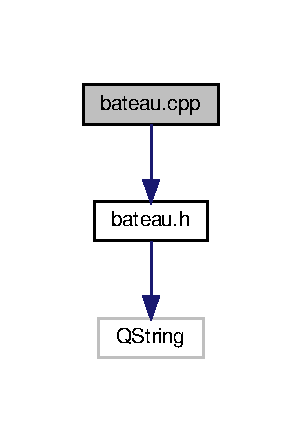
\includegraphics[width=145pt]{bateau_8cpp__incl}
\end{center}
\end{figure}

\hypertarget{bateau_8h}{}\section{Référence du fichier bateau.\+h}
\label{bateau_8h}\index{bateau.\+h@{bateau.\+h}}
{\ttfamily \#include $<$Q\+String$>$}\newline
Graphe des dépendances par inclusion de bateau.\+h\+:\nopagebreak
\begin{figure}[H]
\begin{center}
\leavevmode
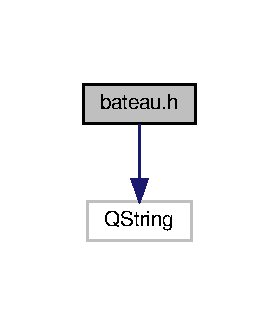
\includegraphics[width=134pt]{bateau_8h__incl}
\end{center}
\end{figure}
Ce graphe montre quels fichiers incluent directement ou indirectement ce fichier \+:\nopagebreak
\begin{figure}[H]
\begin{center}
\leavevmode
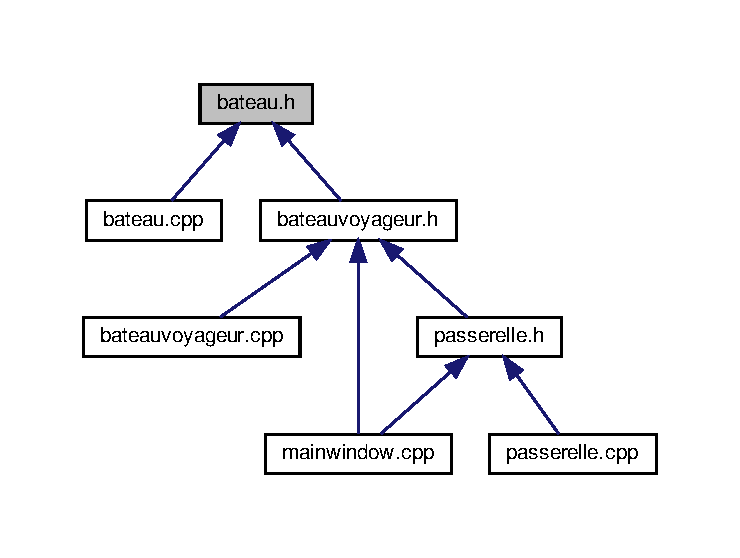
\includegraphics[width=350pt]{bateau_8h__dep__incl}
\end{center}
\end{figure}
\subsection*{Classes}
\begin{DoxyCompactItemize}
\item 
class \hyperlink{class_bateau}{Bateau}
\begin{DoxyCompactList}\small\item\em La classe \hyperlink{class_bateau}{Bateau} C\textquotesingle{}est la classe mère de la classe \hyperlink{class_bateau_voyageur}{Bateau\+Voyageur} Chaque bateau dispose de 4 propriétés. \end{DoxyCompactList}\end{DoxyCompactItemize}

\hypertarget{bateauvoyageur_8cpp}{}\section{Référence du fichier bateauvoyageur.\+cpp}
\label{bateauvoyageur_8cpp}\index{bateauvoyageur.\+cpp@{bateauvoyageur.\+cpp}}
{\ttfamily \#include \char`\"{}bateauvoyageur.\+h\char`\"{}}\newline
Graphe des dépendances par inclusion de bateauvoyageur.\+cpp\+:\nopagebreak
\begin{figure}[H]
\begin{center}
\leavevmode
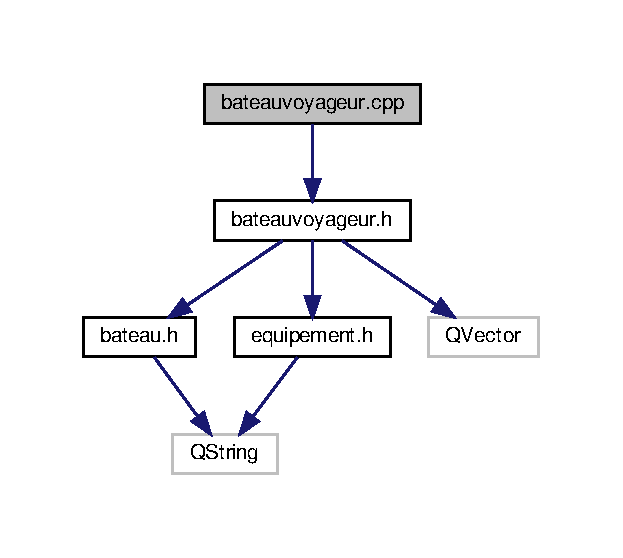
\includegraphics[width=299pt]{bateauvoyageur_8cpp__incl}
\end{center}
\end{figure}

\hypertarget{bateauvoyageur_8h}{}\section{Référence du fichier bateauvoyageur.\+h}
\label{bateauvoyageur_8h}\index{bateauvoyageur.\+h@{bateauvoyageur.\+h}}
{\ttfamily \#include \char`\"{}bateau.\+h\char`\"{}}\newline
{\ttfamily \#include \char`\"{}equipement.\+h\char`\"{}}\newline
{\ttfamily \#include $<$Q\+Vector$>$}\newline
Graphe des dépendances par inclusion de bateauvoyageur.\+h\+:\nopagebreak
\begin{figure}[H]
\begin{center}
\leavevmode
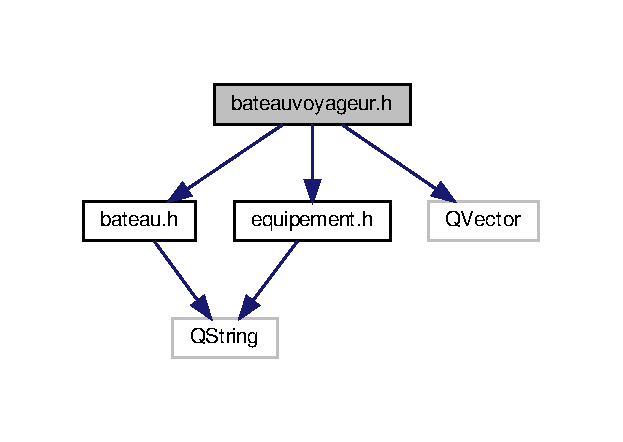
\includegraphics[width=299pt]{bateauvoyageur_8h__incl}
\end{center}
\end{figure}
Ce graphe montre quels fichiers incluent directement ou indirectement ce fichier \+:\nopagebreak
\begin{figure}[H]
\begin{center}
\leavevmode
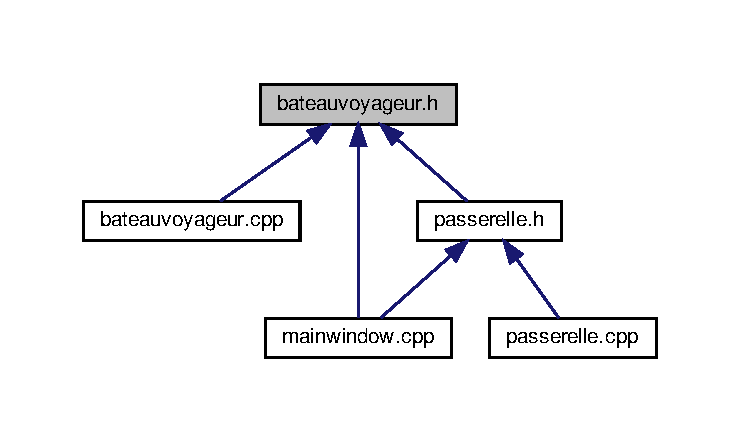
\includegraphics[width=350pt]{bateauvoyageur_8h__dep__incl}
\end{center}
\end{figure}
\subsection*{Classes}
\begin{DoxyCompactItemize}
\item 
class \hyperlink{class_bateau_voyageur}{Bateau\+Voyageur}
\begin{DoxyCompactList}\small\item\em La classe \hyperlink{class_bateau_voyageur}{Bateau\+Voyageur} C\textquotesingle{}est une dépendance de la classe \hyperlink{class_passerelle}{Passerelle} Chaque bateau voyageur dispose de 3 propriétés. \end{DoxyCompactList}\end{DoxyCompactItemize}

\hypertarget{equipement_8cpp}{}\section{Référence du fichier equipement.\+cpp}
\label{equipement_8cpp}\index{equipement.\+cpp@{equipement.\+cpp}}
{\ttfamily \#include \char`\"{}equipement.\+h\char`\"{}}\newline
Graphe des dépendances par inclusion de equipement.\+cpp\+:\nopagebreak
\begin{figure}[H]
\begin{center}
\leavevmode
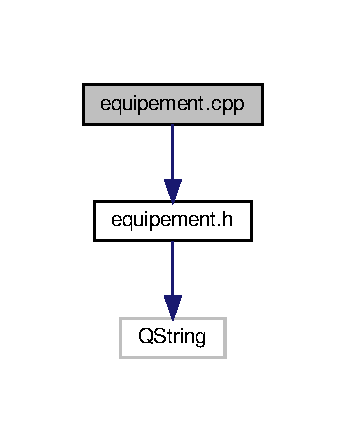
\includegraphics[width=166pt]{equipement_8cpp__incl}
\end{center}
\end{figure}

\hypertarget{equipement_8h}{}\section{Référence du fichier equipement.\+h}
\label{equipement_8h}\index{equipement.\+h@{equipement.\+h}}
{\ttfamily \#include $<$Q\+String$>$}\newline
Graphe des dépendances par inclusion de equipement.\+h\+:\nopagebreak
\begin{figure}[H]
\begin{center}
\leavevmode
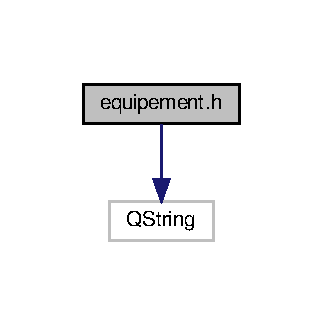
\includegraphics[width=155pt]{equipement_8h__incl}
\end{center}
\end{figure}
Ce graphe montre quels fichiers incluent directement ou indirectement ce fichier \+:\nopagebreak
\begin{figure}[H]
\begin{center}
\leavevmode
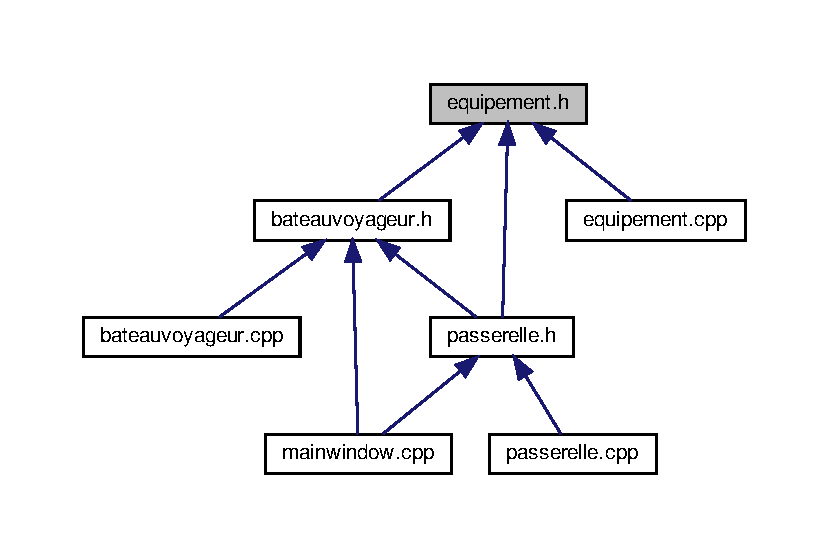
\includegraphics[width=350pt]{equipement_8h__dep__incl}
\end{center}
\end{figure}
\subsection*{Classes}
\begin{DoxyCompactItemize}
\item 
class \hyperlink{class_equipement}{Equipement}
\begin{DoxyCompactList}\small\item\em La classe \hyperlink{class_equipement}{Equipement} C\textquotesingle{}est une dépendance de la classe \hyperlink{class_passerelle}{Passerelle} Chaque équipement possède 2 propriétés. \end{DoxyCompactList}\end{DoxyCompactItemize}

\hypertarget{jeuenregistrement_8cpp}{}\section{Référence du fichier jeuenregistrement.\+cpp}
\label{jeuenregistrement_8cpp}\index{jeuenregistrement.\+cpp@{jeuenregistrement.\+cpp}}
{\ttfamily \#include \char`\"{}jeuenregistrement.\+h\char`\"{}}\newline
Graphe des dépendances par inclusion de jeuenregistrement.\+cpp\+:\nopagebreak
\begin{figure}[H]
\begin{center}
\leavevmode
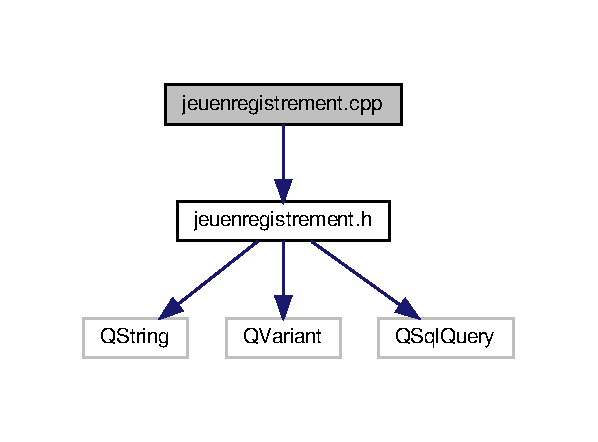
\includegraphics[width=287pt]{jeuenregistrement_8cpp__incl}
\end{center}
\end{figure}

\hypertarget{jeuenregistrement_8h}{}\section{Référence du fichier jeuenregistrement.\+h}
\label{jeuenregistrement_8h}\index{jeuenregistrement.\+h@{jeuenregistrement.\+h}}
{\ttfamily \#include $<$Q\+String$>$}\newline
{\ttfamily \#include $<$Q\+Variant$>$}\newline
{\ttfamily \#include $<$Q\+Sql\+Query$>$}\newline
Graphe des dépendances par inclusion de jeuenregistrement.\+h\+:\nopagebreak
\begin{figure}[H]
\begin{center}
\leavevmode
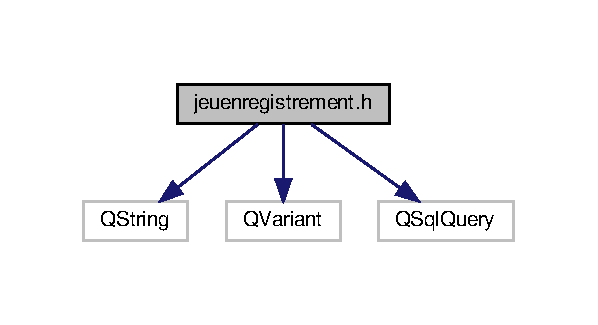
\includegraphics[width=287pt]{jeuenregistrement_8h__incl}
\end{center}
\end{figure}
Ce graphe montre quels fichiers incluent directement ou indirectement ce fichier \+:\nopagebreak
\begin{figure}[H]
\begin{center}
\leavevmode
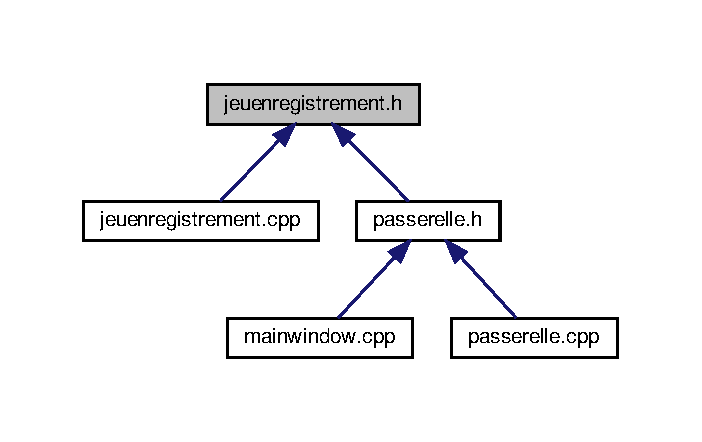
\includegraphics[width=337pt]{jeuenregistrement_8h__dep__incl}
\end{center}
\end{figure}
\subsection*{Classes}
\begin{DoxyCompactItemize}
\item 
class \hyperlink{class_jeu_enregistrement}{Jeu\+Enregistrement}
\begin{DoxyCompactList}\small\item\em La classe \hyperlink{class_jeu_enregistrement}{Jeu\+Enregistrement} Elle hérite de la classe Q\+Sql\+Query Elle permet de manipuler un jeu de données. \end{DoxyCompactList}\end{DoxyCompactItemize}

\hypertarget{main_8cpp}{}\section{Référence du fichier main.\+cpp}
\label{main_8cpp}\index{main.\+cpp@{main.\+cpp}}
{\ttfamily \#include \char`\"{}mainwindow.\+h\char`\"{}}\newline
{\ttfamily \#include $<$Q\+Application$>$}\newline
{\ttfamily \#include $<$Q\+Sql\+Database$>$}\newline
Graphe des dépendances par inclusion de main.\+cpp\+:\nopagebreak
\begin{figure}[H]
\begin{center}
\leavevmode
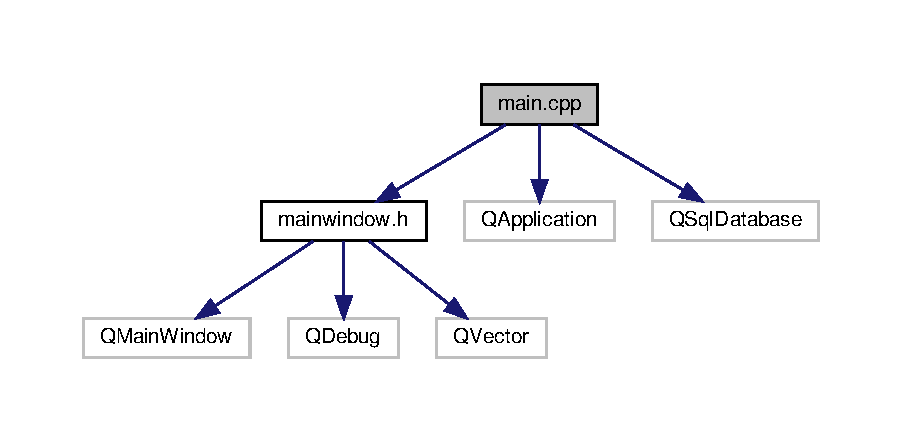
\includegraphics[width=350pt]{main_8cpp__incl}
\end{center}
\end{figure}
\subsection*{Fonctions}
\begin{DoxyCompactItemize}
\item 
int \hyperlink{main_8cpp_a0ddf1224851353fc92bfbff6f499fa97}{main} (int argc, char $\ast$argv\mbox{[}$\,$\mbox{]})
\begin{DoxyCompactList}\small\item\em main Fonction principale qui permet de lancer l\textquotesingle{}application \end{DoxyCompactList}\end{DoxyCompactItemize}


\subsection{Documentation des fonctions}
\mbox{\Hypertarget{main_8cpp_a0ddf1224851353fc92bfbff6f499fa97}\label{main_8cpp_a0ddf1224851353fc92bfbff6f499fa97}} 
\index{main.\+cpp@{main.\+cpp}!main@{main}}
\index{main@{main}!main.\+cpp@{main.\+cpp}}
\subsubsection{\texorpdfstring{main()}{main()}}
{\footnotesize\ttfamily int main (\begin{DoxyParamCaption}\item[{int}]{argc,  }\item[{char $\ast$}]{argv\mbox{[}$\,$\mbox{]} }\end{DoxyParamCaption})}



main Fonction principale qui permet de lancer l\textquotesingle{}application 


\begin{DoxyParams}{Paramètres}
{\em argc} & int \\
\hline
{\em argv} & char \\
\hline
\end{DoxyParams}
\begin{DoxyReturn}{Renvoie}
La fenêtre de l\textquotesingle{}application 
\end{DoxyReturn}


Définition à la ligne 12 du fichier main.\+cpp.


\hypertarget{mainwindow_8cpp}{}\section{Référence du fichier mainwindow.\+cpp}
\label{mainwindow_8cpp}\index{mainwindow.\+cpp@{mainwindow.\+cpp}}
{\ttfamily \#include \char`\"{}mainwindow.\+h\char`\"{}}\newline
{\ttfamily \#include \char`\"{}ui\+\_\+mainwindow.\+h\char`\"{}}\newline
{\ttfamily \#include \char`\"{}pdf.\+h\char`\"{}}\newline
{\ttfamily \#include \char`\"{}bateauvoyageur.\+h\char`\"{}}\newline
{\ttfamily \#include \char`\"{}passerelle.\+h\char`\"{}}\newline
Graphe des dépendances par inclusion de mainwindow.\+cpp\+:\nopagebreak
\begin{figure}[H]
\begin{center}
\leavevmode
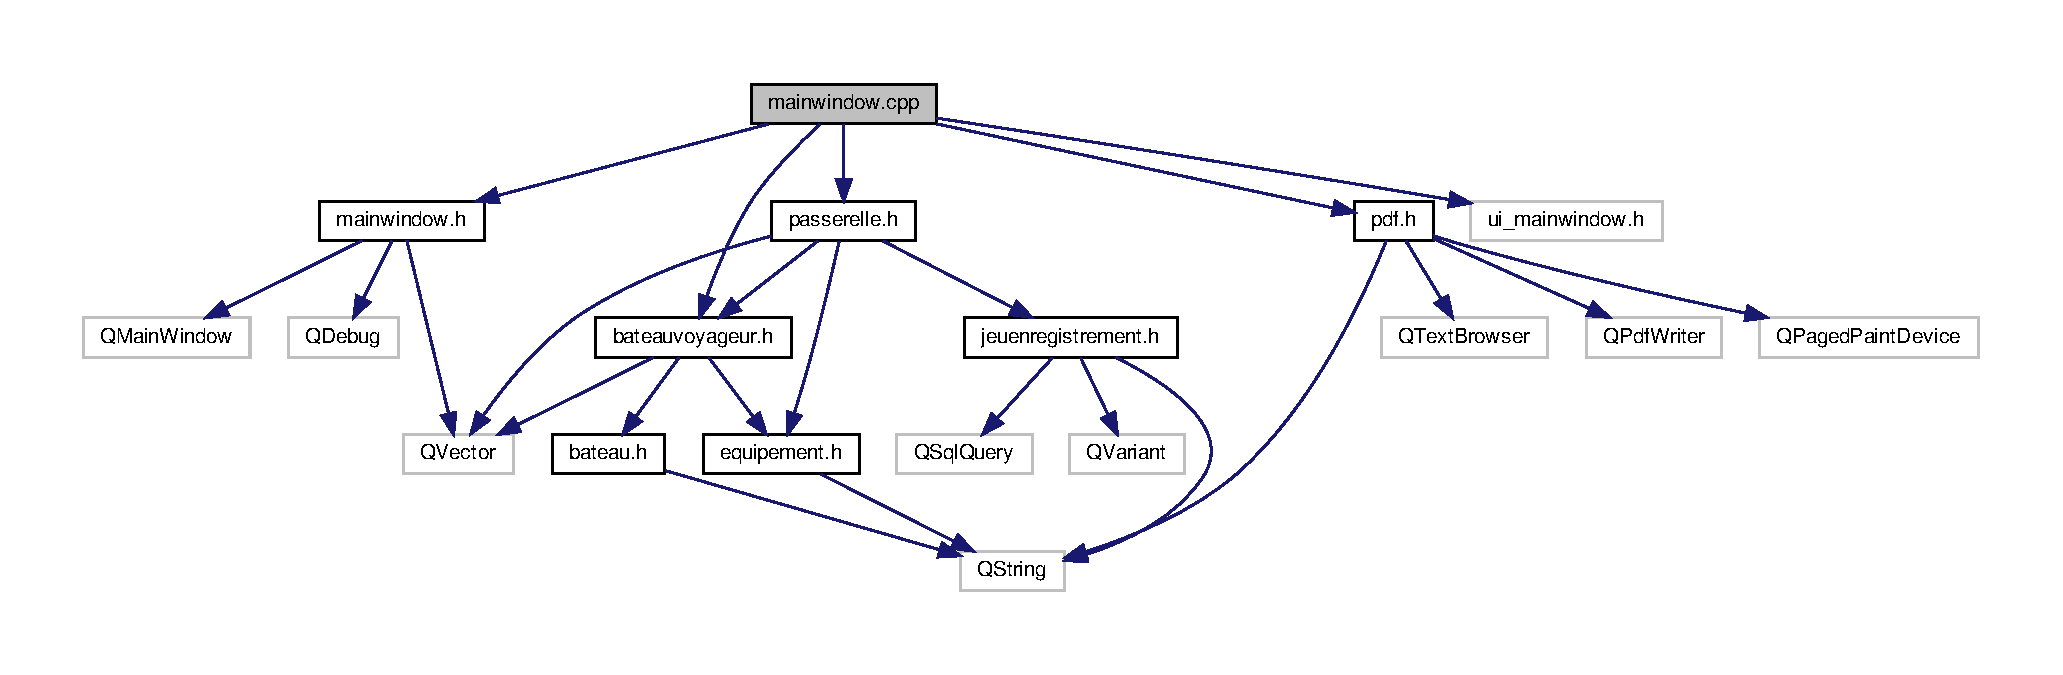
\includegraphics[width=350pt]{mainwindow_8cpp__incl}
\end{center}
\end{figure}

\hypertarget{mainwindow_8h}{}\section{Référence du fichier mainwindow.\+h}
\label{mainwindow_8h}\index{mainwindow.\+h@{mainwindow.\+h}}
{\ttfamily \#include $<$Q\+Main\+Window$>$}\newline
{\ttfamily \#include $<$Q\+Debug$>$}\newline
{\ttfamily \#include $<$Q\+Vector$>$}\newline
Graphe des dépendances par inclusion de mainwindow.\+h\+:\nopagebreak
\begin{figure}[H]
\begin{center}
\leavevmode
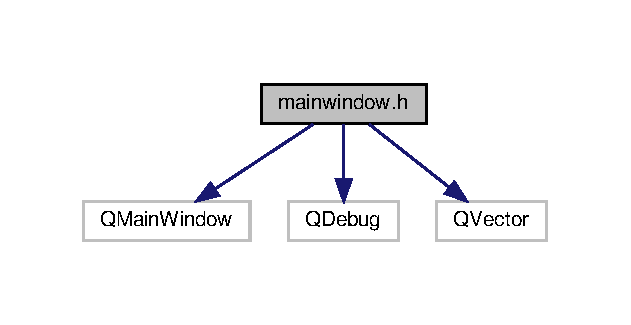
\includegraphics[width=303pt]{mainwindow_8h__incl}
\end{center}
\end{figure}
Ce graphe montre quels fichiers incluent directement ou indirectement ce fichier \+:\nopagebreak
\begin{figure}[H]
\begin{center}
\leavevmode
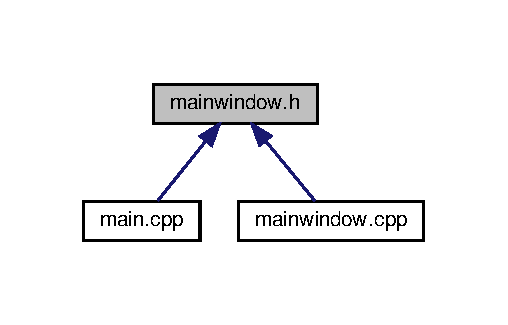
\includegraphics[width=244pt]{mainwindow_8h__dep__incl}
\end{center}
\end{figure}
\subsection*{Classes}
\begin{DoxyCompactItemize}
\item 
class \hyperlink{class_main_window}{Main\+Window}
\begin{DoxyCompactList}\small\item\em La classe \hyperlink{class_main_window}{Main\+Window} Elle hérite de la classe Q\+Main\+Window Elle permet de créer la fenêtre de l\textquotesingle{}application. \end{DoxyCompactList}\end{DoxyCompactItemize}
\subsection*{Espaces de nommage}
\begin{DoxyCompactItemize}
\item 
 \hyperlink{namespace_ui}{Ui}
\end{DoxyCompactItemize}

\hypertarget{passerelle_8cpp}{}\section{Référence du fichier passerelle.\+cpp}
\label{passerelle_8cpp}\index{passerelle.\+cpp@{passerelle.\+cpp}}
{\ttfamily \#include \char`\"{}passerelle.\+h\char`\"{}}\newline
{\ttfamily \#include $<$Q\+Debug$>$}\newline
Graphe des dépendances par inclusion de passerelle.\+cpp\+:\nopagebreak
\begin{figure}[H]
\begin{center}
\leavevmode
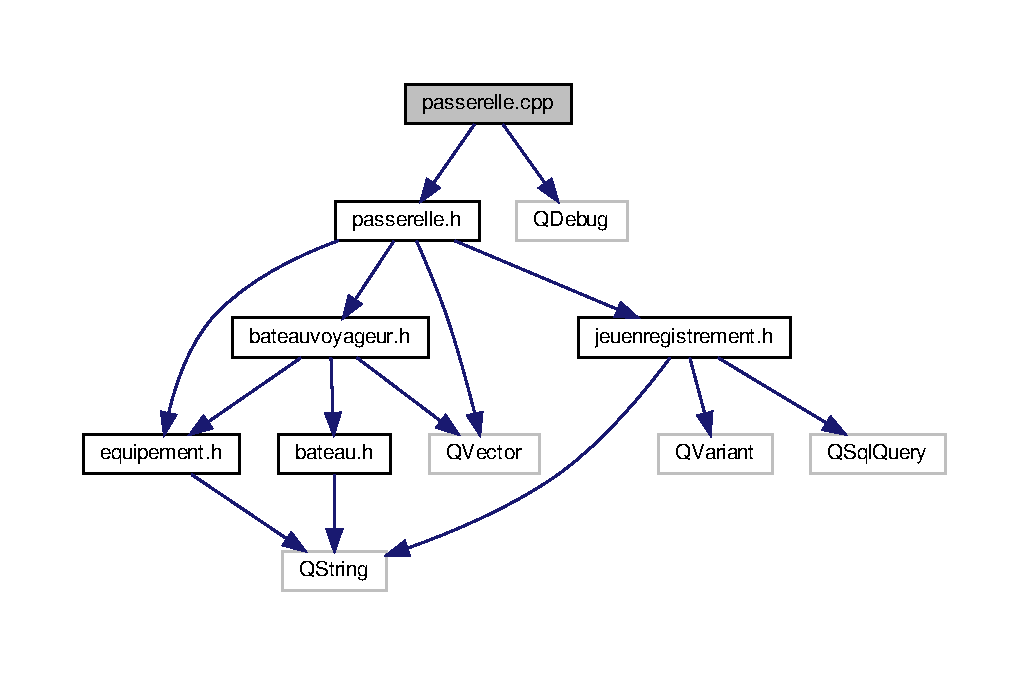
\includegraphics[width=350pt]{passerelle_8cpp__incl}
\end{center}
\end{figure}

\hypertarget{passerelle_8h}{}\section{Référence du fichier passerelle.\+h}
\label{passerelle_8h}\index{passerelle.\+h@{passerelle.\+h}}
{\ttfamily \#include \char`\"{}bateauvoyageur.\+h\char`\"{}}\newline
{\ttfamily \#include \char`\"{}equipement.\+h\char`\"{}}\newline
{\ttfamily \#include \char`\"{}jeuenregistrement.\+h\char`\"{}}\newline
{\ttfamily \#include $<$Q\+Vector$>$}\newline
Graphe des dépendances par inclusion de passerelle.\+h\+:\nopagebreak
\begin{figure}[H]
\begin{center}
\leavevmode
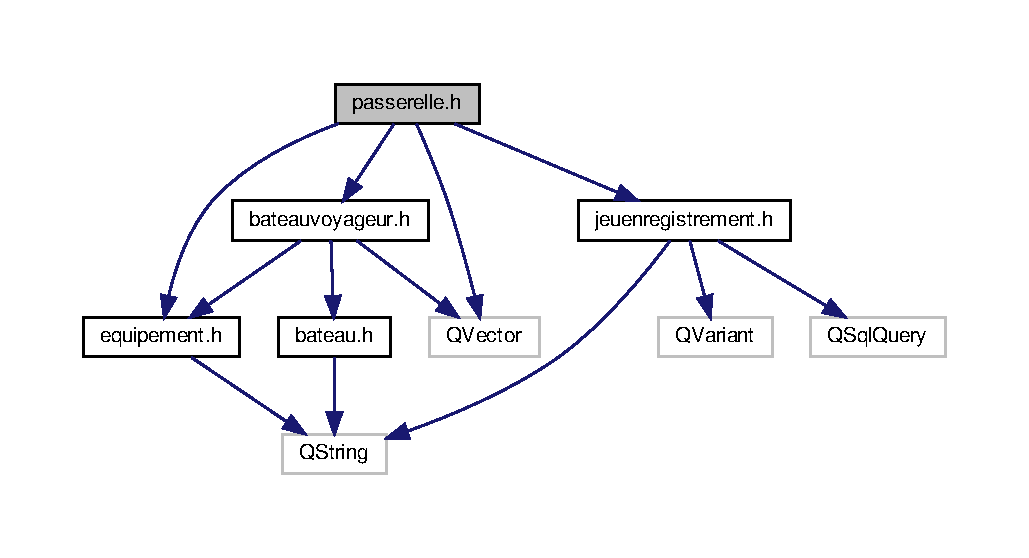
\includegraphics[width=350pt]{passerelle_8h__incl}
\end{center}
\end{figure}
Ce graphe montre quels fichiers incluent directement ou indirectement ce fichier \+:\nopagebreak
\begin{figure}[H]
\begin{center}
\leavevmode
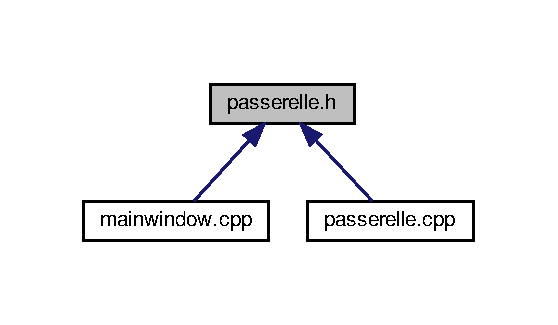
\includegraphics[width=268pt]{passerelle_8h__dep__incl}
\end{center}
\end{figure}
\subsection*{Classes}
\begin{DoxyCompactItemize}
\item 
class \hyperlink{class_passerelle}{Passerelle}
\begin{DoxyCompactList}\small\item\em La classe \hyperlink{class_passerelle}{Passerelle} Elle est dépendante des classes \hyperlink{class_bateau_voyageur}{Bateau\+Voyageur} et \hyperlink{class_equipement}{Equipement}. \end{DoxyCompactList}\end{DoxyCompactItemize}

\hypertarget{pdf_8cpp}{}\section{Référence du fichier pdf.\+cpp}
\label{pdf_8cpp}\index{pdf.\+cpp@{pdf.\+cpp}}
{\ttfamily \#include \char`\"{}pdf.\+h\char`\"{}}\newline
Graphe des dépendances par inclusion de pdf.\+cpp\+:\nopagebreak
\begin{figure}[H]
\begin{center}
\leavevmode
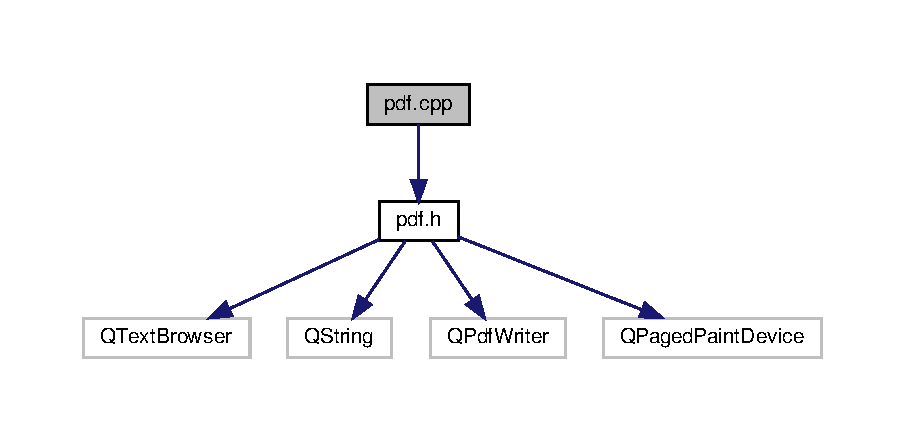
\includegraphics[width=350pt]{pdf_8cpp__incl}
\end{center}
\end{figure}

\hypertarget{pdf_8h}{}\section{Référence du fichier pdf.\+h}
\label{pdf_8h}\index{pdf.\+h@{pdf.\+h}}
{\ttfamily \#include $<$Q\+Text\+Browser$>$}\newline
{\ttfamily \#include $<$Q\+String$>$}\newline
{\ttfamily \#include $<$Q\+Pdf\+Writer$>$}\newline
{\ttfamily \#include $<$Q\+Paged\+Paint\+Device$>$}\newline
Graphe des dépendances par inclusion de pdf.\+h\+:\nopagebreak
\begin{figure}[H]
\begin{center}
\leavevmode
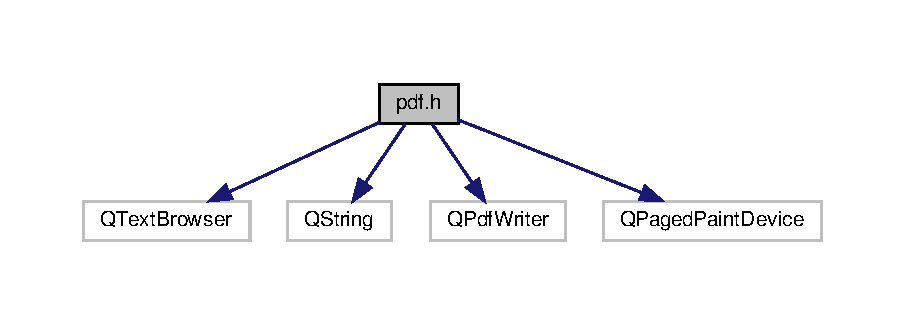
\includegraphics[width=350pt]{pdf_8h__incl}
\end{center}
\end{figure}
Ce graphe montre quels fichiers incluent directement ou indirectement ce fichier \+:\nopagebreak
\begin{figure}[H]
\begin{center}
\leavevmode
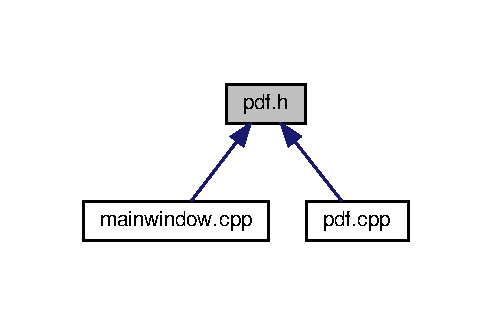
\includegraphics[width=236pt]{pdf_8h__dep__incl}
\end{center}
\end{figure}
\subsection*{Classes}
\begin{DoxyCompactItemize}
\item 
class \hyperlink{class_p_d_f}{P\+DF}
\begin{DoxyCompactList}\small\item\em La classe \hyperlink{class_p_d_f}{P\+DF} Elle hérite de la classe Q\+Text\+Browser Elle permet de générer un document \hyperlink{class_p_d_f}{P\+DF} Chaque pdf d\textquotesingle{}une propriété \end{DoxyCompactList}\end{DoxyCompactItemize}

%--- End generated contents ---

% Index
\backmatter
\newpage
\phantomsection
\clearemptydoublepage
\addcontentsline{toc}{chapter}{Index}
\printindex

\end{document}
